\chapter{\todo{Higher Order Fields}}
\thumbforchapter{}
%\chaptertoc{}
%\newpage


%====================
% 	Introduction
%====================
\section{\review{Introduction}}

Beam-based high order field measurements have been carried out in the LHC since its first
Run~\cite{maclean_non-linear_2011, maclean_commissioning_2016-1}, via
chromaticity studies. Those measurements, made by varying the RF frequency while observing the
resulting tune change, have been performed with a momentum offset of up to $\delta = \pm 2.2 \times
10^{-3}$, which led to the observation of the third order term of the non-linear chromaticity.

During the commissioning of Run~3 in 2022, a new collimator sequence has been introduced, allowing wider
momentum offset measurements, within $\delta \in [-3.2\times 10^{-3},3.7 \times 10^{-3}]$. This
improved setup led to the observation of the fourth and fifth order terms at injection energy.
Those terms, denoted $Q^{(4)}$ and $Q^{(5)}$ respectively in
\cref{eq:very_high_orders:chromaticity_high_orders}, are produced to first order by dodecapoles and
decatetrapoles. Dodecapoles being powered off at injection and decatetrapoles being absent from the
lattice, those fields originate from the field errors of the various magnets installed in the LHC.

\begin{equation}
  \begin{aligned}
    Q(\delta) = Q_0 + Q'\delta &+ \frac{1}{2!}Q''\delta^2 + \frac{1}{3!}Q'''\delta^3
                                + \frac{1}{4!}Q^{(4)}\delta^4  + \frac{1}{5!}Q^{(5)}\delta^5
                                + \mathcal{O}(\delta^6).
  \end{aligned}
  \label{eq:very_high_orders:chromaticity_high_orders}
\end{equation}


In addition to completing the measurements of high-order fields through chromaticity scans,
turn-by-turn measurements were also conducted. High amplitude kicks indeed made it possible to
observe dodecapolar RDTs in the LHC for the first time. Such fields were never before observed
directly, but rather only via feed-down to amplitude detuning~\cite{dilly_corrections_2022}.



%=============================
%        Chromaticity
%=============================
\section{\review{Chromaticity}}
\label{section:very_hgih_orders:chromaticity}

As described in \cref{subsection:optics_corrections_chromaticity}, the momentum offset $\delta$ is
related to the RF frequency and the momentum compaction factor. This relation is given as a
simplified form in \cref{eq:very_high_orders:simplified_eq_momentum_compaction}, neglecting the
Lorentz factor $\gamma$. 
The model $\alpha_c$ for the LHC injection optics is $3.48 \times 10^{-4}$ for beam 1 and $3.47
\times 10^{-4}$ for beam 2. Via this relation, a change of 140Hz of the RF frequency corresponds to
a momentum offset of about $-0.001$.

\begin{equation}
    \delta = -\frac{1}{\alpha_c} \cdot \frac{\Delta f_{RF}}{f_{RF,nominal}}.
    \label{eq:very_high_orders:simplified_eq_momentum_compaction}
\end{equation}

The RF frequency is thus varied to induce a change in momentum-offset. The tune will then vary with
this momentum-offset, as shows the chromaticity function expanded up to the fifth order,

\begin{equation}
  \begin{aligned}
    Q(\delta) = Q_0 + Q'\delta &+ \frac{1}{2!}Q''\delta^2 + \frac{1}{3!}Q'''\delta^3
                                + \frac{1}{4!}Q^{(4)}\delta^4  + \frac{1}{5!}Q^{(5)}\delta^5
                                + \mathcal{O}(\delta^6).
  \end{aligned}
  \label{eq:very_high_orders:chromaticity_high_orders}
\end{equation}

%\begin{figure}[tbh]
%    \centering
%    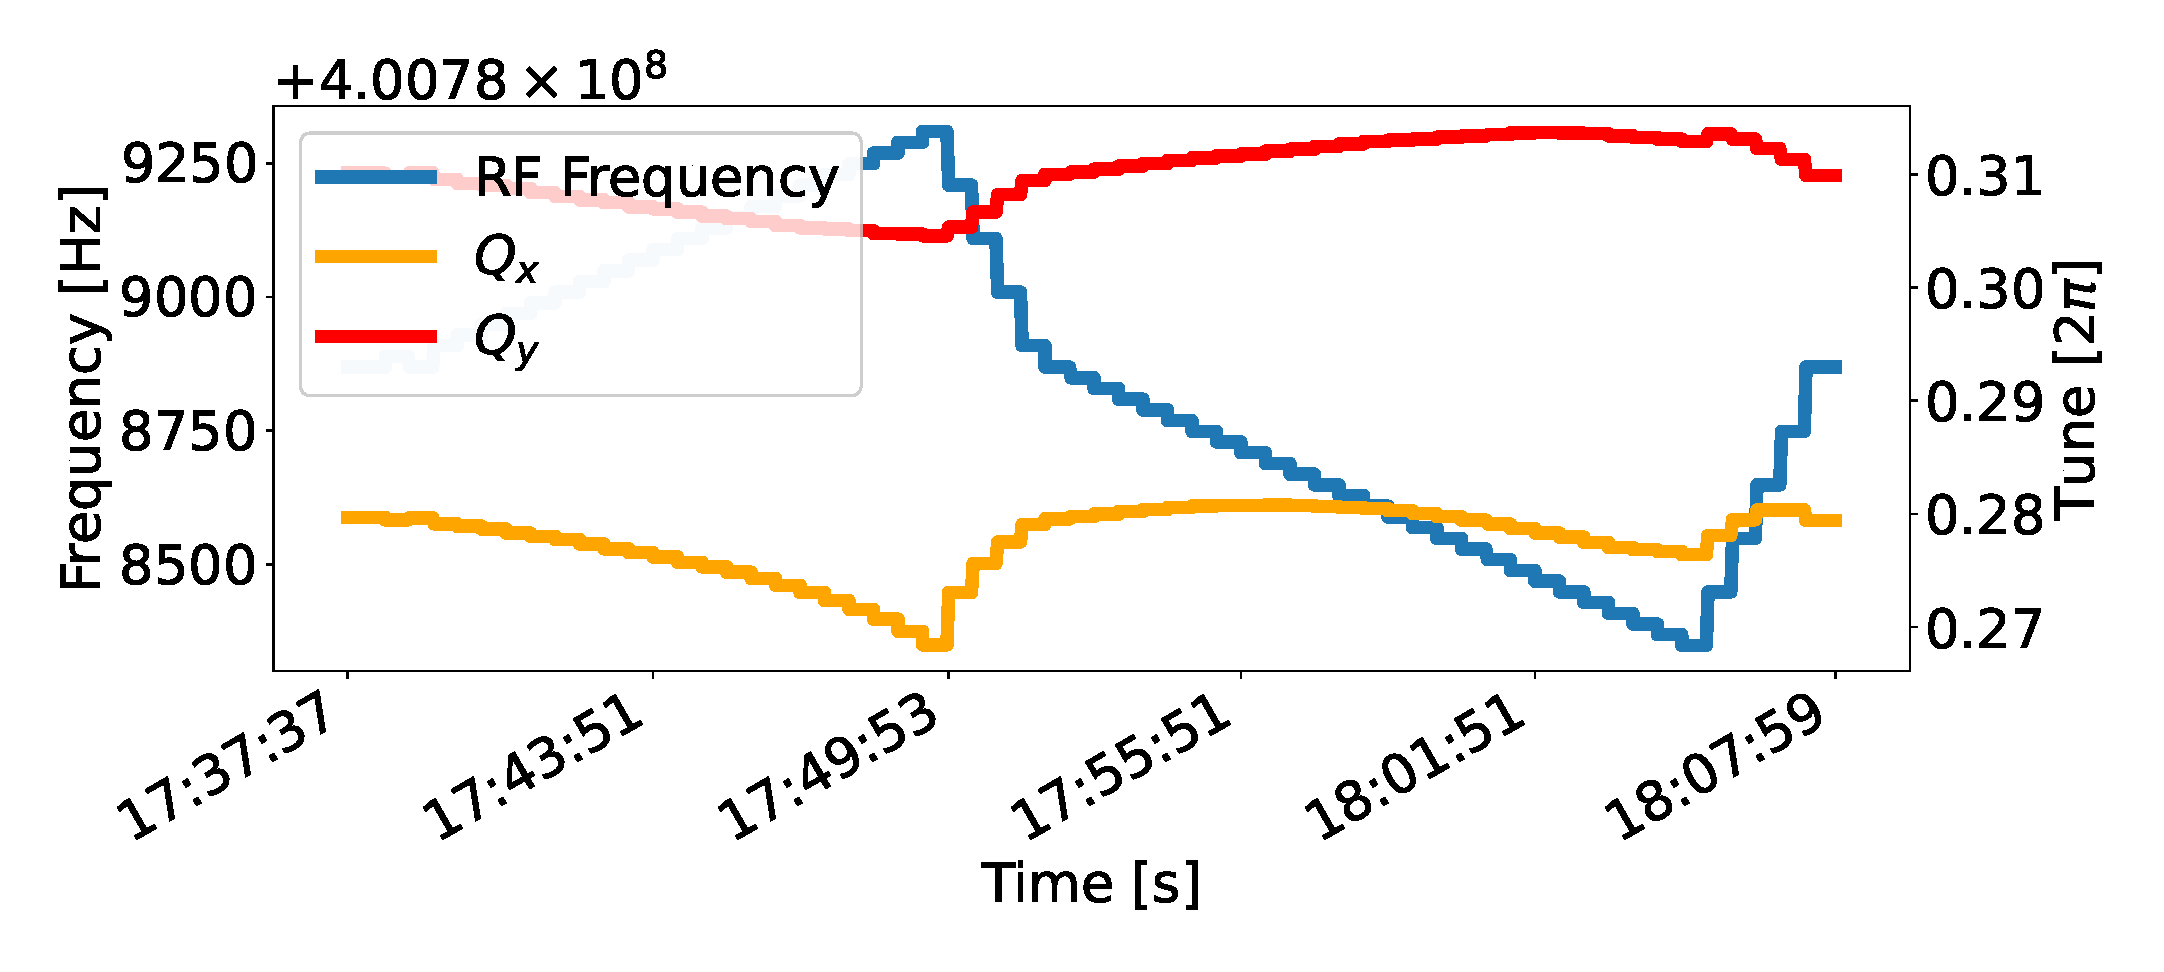
\includegraphics[width=\columnwidth]{images/MOPL027_f1-1.pdf}
%    \caption{Observation of the tune dependence on momentum offset, created by a shift of RF frequency.}
%    \label{fig:very_high_orders:rf_scan}
%\end{figure}

%To properly characterize higher orders of the chromaticity function and ensure quality measurements,
%several steps are required. The tune measured during chromaticity scans can exhibit jitter and
%resonance lines may appear, requiring thorough data cleaning to either reject problematic data
%points or reduce error bars. The simplified
%\cref{eq:very_high_orders:simplified_eq_momentum_compaction}, describing $\delta$, has been
%sufficient for reliably measuring up to the third order chromaticity. However, this relation also
%needs verification.




%------------------------------------------
%            First Measurement
%------------------------------------------
\FloatBarrier
\subsection{\review{First Observation}}

Before focusing on the measurement of higher-order chromaticity such as $Q^{(5)}$, it is essential
to consider the procedural improvements that enable such measurements. Improvements in dynamic
aperture, collimation and signal processing with noise reduction now allow for larger oscillation
amplitudes and enhancements in the precision of measurements across broader amplitude ranges. This
increased resolution facilitates the study of non-linear chromaticity, which has been extended to
include higher-order terms, making it possible to detect contributions from dodecapolar and
decatetrapolar fields.
These developments are particularly interesting because they suggest the possibility of directly
measuring $Q^{(5)}$, an observable previously inaccessible due to narrower momentum offset ranges.


A measurement was performed with the octupolar and decapolar correctors \textit{MCO} and
\textit{MCD} set to their nominal settings. These are aimed at correcting $Q''$ and $Q'''$, as
previously described in \cref{chapter:decapoles}. Results of this initial measurement are shown in
\cref{tab:high_orders:chroma_fidel}. Lower order chromaticities such as $Q'$ and $Q''$ are
consistent with measurements done during the previous Run~\cite{maclean_commissioning_2016}.
The fourth and fifth order chromaticities, $Q^{(4)}$ and $Q^{(5)}$, are primarily expected
to originate from dodecapolar errors in the quadrupoles and decatetrapolar errors in the main
dipoles, respectively, as given by the following expressions:

\begin{equation}
    \begin{aligned}
        &\Delta Q_x^{(4)} =  \frac{1}{4\pi} K_{6} L \beta_x D_x^{4}, 
        &&\Delta Q_x^{(5)} =  \frac{1}{4\pi} K_{7} L \beta_x D_x^{5},&&\\
        %
        &\Delta Q_y^{(4)} = -\frac{1}{4\pi} K_{6} L \beta_x D_x^{4},
        &&\Delta Q_x^{(5)} = -\frac{1}{4\pi} K_{7} L \beta_x D_x^{5}.
    \end{aligned}
    %\label{eq:detuning_effects:chromaticity_strength}
\end{equation}


\begin{table}[!htb]
    \centering
    \begin{tabular}{lrrrr}
    \toprule
         Plane & $Q^{(2)} [10^3]$ & $Q^{(3)} [10^6]$ & $Q^{(4)} [10^9]$ & $Q^{(5)} [10^{12}]$ \\
    \midrule
        Beam 1 &              &               &              & \\
        \hspace{2mm}X         & $-2.44 \pm 0.02$ & $-3.36 \pm 0.04$ & $-0.56 \pm 0.02 $ & $ 1.20 \pm 0.07$ \\
        \hspace{2mm}Y         & $ 0.97 \pm 0.02$ & $ 1.62 \pm 0.05$ &$  0.15 \pm 0.03$ & $-0.88 \pm 0.09$ \\
        Beam 2 &              &                &                & \\
        \hspace{2mm}X         & $-2.45 \pm 0.03$ & $-2.72 \pm 0.08$ & $-1.00 \pm 0.05 $ & $ 0.15 \pm 0.14$ \\
        \hspace{2mm}Y         & $ 0.79 \pm 0.03$ & $1.54 \pm 0.06 $ & $ 0.24 \pm 0.04 $ & $-0.74 \pm 0.13$ \\
    \bottomrule
    \end{tabular}
    \caption{Terms of the high order chromaticity obtained during Run~3's commissioning in 2022,
    with nominal corrections.}
    \label{tab:high_orders:chroma_fidel}
  \end{table}

Due to the RF-scan method, the momentum offset crosses zero multiple times during the measurement.
The absence of tune change at these points allows to conclude that the tune drift throughout
the measurement is negligible. This measurement was conducted after an extended period at
injection energy, where the decay of the sextupolar fields is minimal, causing no significant change
in first-order chromaticity. The fitted curve for the chromaticity function is shown in
\cref{fig:high_orders:chroma_before_correction}, where it is evident that a higher-order polynomial
provides a better fit.

\begin{figure}[!htb]
    \begin{subfigure}{0.49\textwidth}
        \centering
        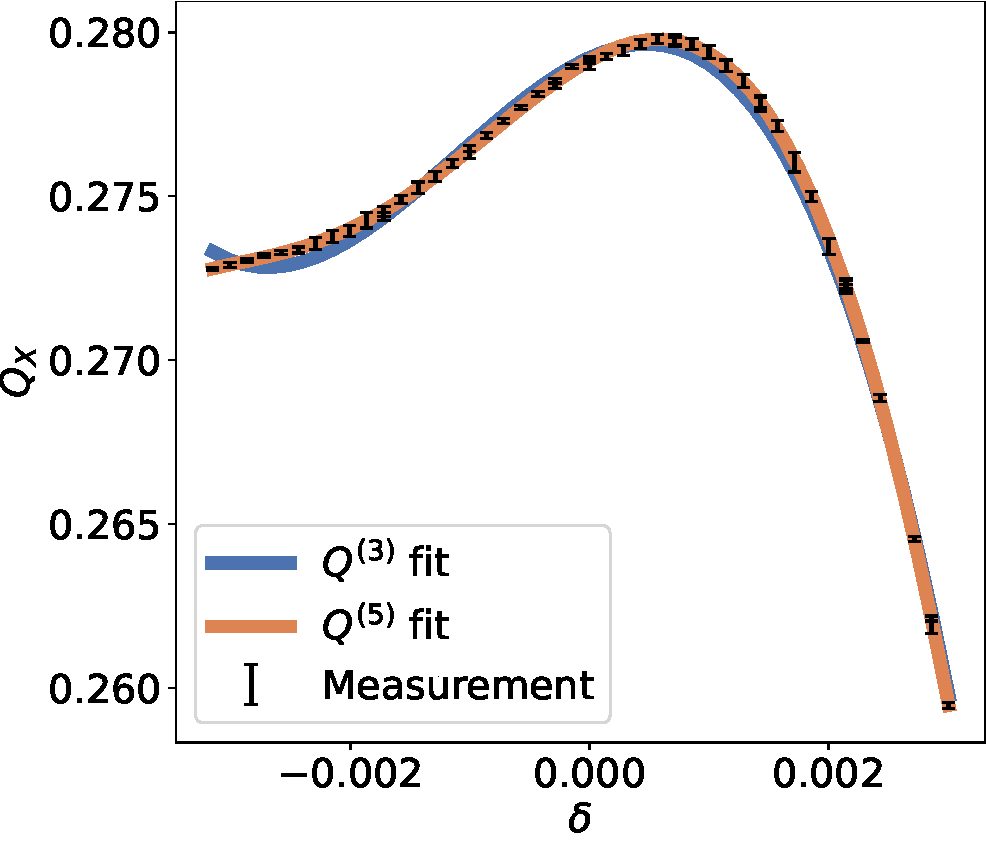
\includegraphics[width=\textwidth]{./images/higher_orders/fidel_chroma/Beam1_Qx.pdf}
        \caption{$Q_x$ Beam 1}
    \end{subfigure}
    \hfill
    \begin{subfigure}{0.49\textwidth}
        \centering
        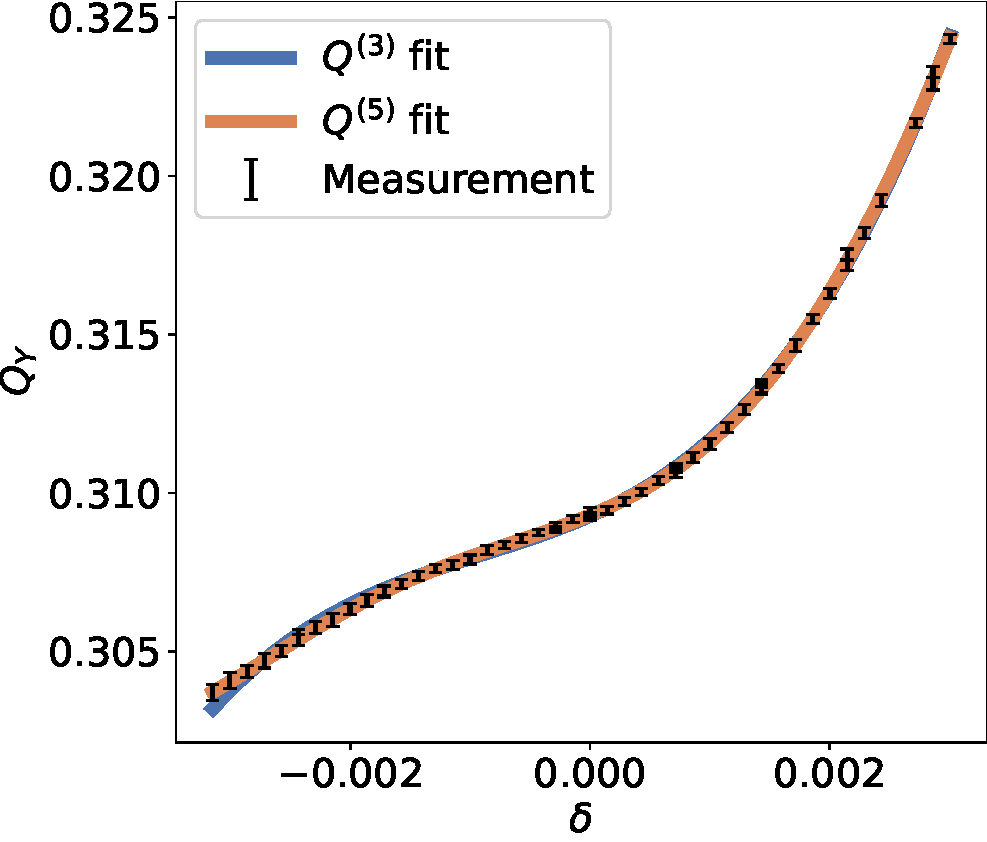
\includegraphics[width=\textwidth]{./images/higher_orders/fidel_chroma/Beam1_Qy.pdf}
        \caption{$Q_y$ Beam 1}
    \end{subfigure}
    %
    \\
    %
    \begin{subfigure}{0.49\textwidth}
        \centering
        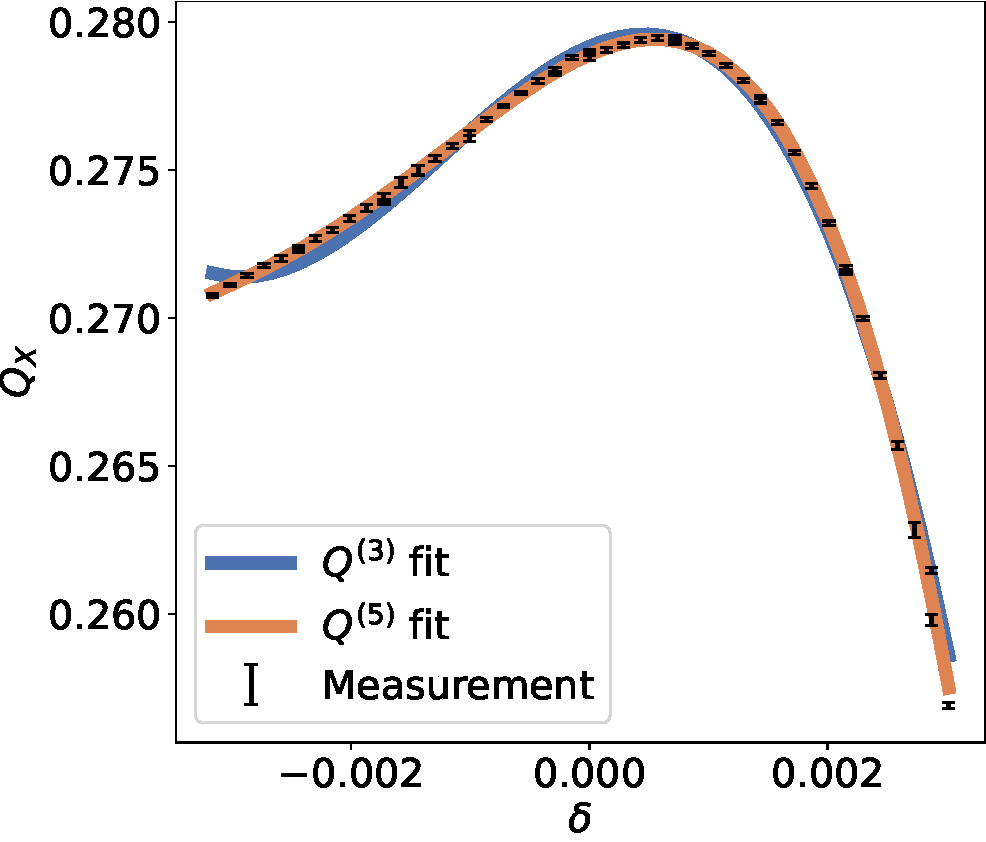
\includegraphics[width=\textwidth]{./images/higher_orders/fidel_chroma/Beam2_Qx.pdf}
        \caption{$Q_x$ Beam 2}
    \end{subfigure}
    \hfill
    \begin{subfigure}{0.49\textwidth}
        \centering
        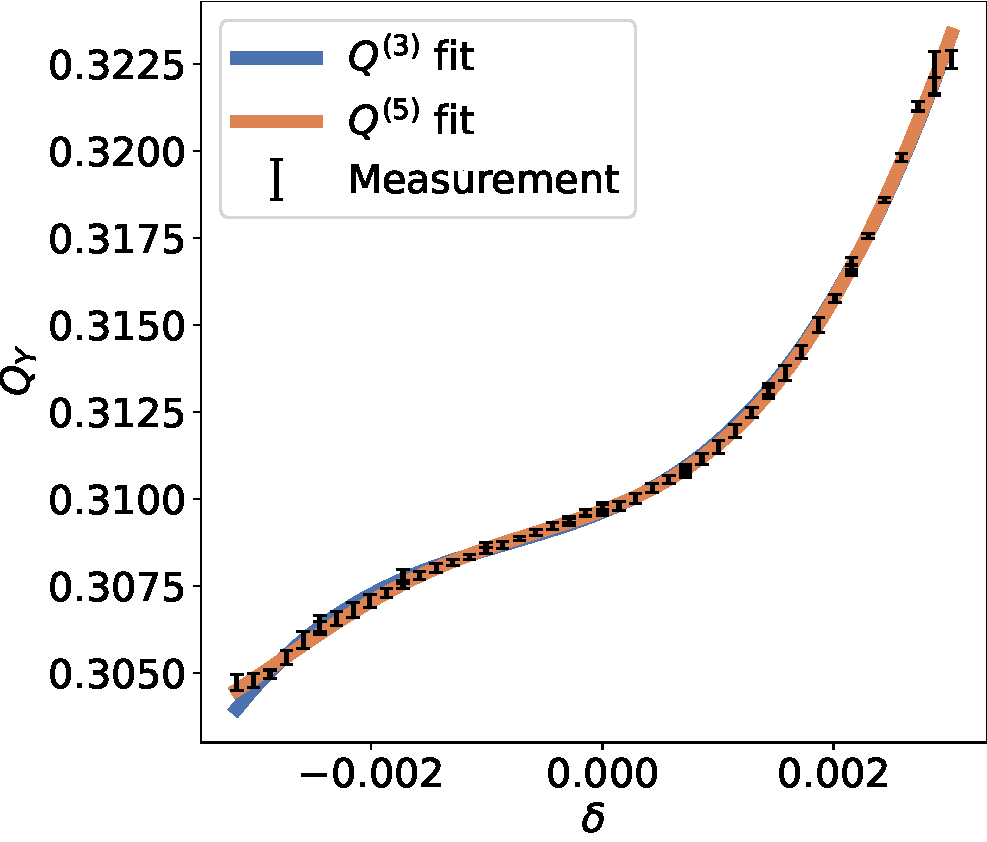
\includegraphics[width=\textwidth]{./images/higher_orders/fidel_chroma/Beam2_Qy.pdf}
        \caption{$Q_y$ Beam 2}
    \end{subfigure}
    \caption{Measurement of higher order chromaticity terms with nominal corrections used
    during operation. Fits are up to the third and fifth order.}
    \label{fig:high_orders:chroma_before_correction}
\end{figure}





%----------------------------------------
%             Fit Quality
%----------------------------------------
%\subsubsection{\review{Fit Quality}}
%\label{subsection:q4q5_quality}

%The values measured for $Q^{(4)}$ and $Q^{(5)}$ are similar across the measurements, with
%nominal and beam-based corrections performed with very different lower order chromaticity, and well 
%separated in time.
%This reproducibility with varying configurations gives confidence that the measured values are
%robust. It is to be noted that one exception exists for the first measurement, the horizontal plane
%of beam 2 showed a high correlation between the fourth and fifth order terms, making the fit less
%reliable.

The reduced chi-square for this measurement of 2022 for each fit order is detailed in
\cref{tab:high_orders:chisquare_quality}. A value of $1$ indicates a good fit. Values above indicate
a poor fit while values below show an over-fit of the data.
While adding terms to the chromaticity function is beneficial to the fit, it can be seen that the
reduced chi-square does not substantially improve above the fifth order, indicating that such
further orders are not warranted.
%\Cref{chroma_comparison} shows a comparison of the measured chromaticity before and after
%beam-based corrections for the horizontal axis of beam 1.

\begin{table}[!htb]
    \centering
    \begin{tabular}{lrrrr}
     \toprule
                  & \multicolumn{4}{c}{$\chi^2_\nu$} \\
      %\cmidrule{2-5}
        Plane     &   $Q^{(3)}$ &  $Q^{(4)}$ &   $Q^{(5)}$ &   $Q^{(6)}$  \\
      \midrule
        Beam 1    &   &   &   & \\
        % The commented out lines are from measurement with the regular BBQ data
        % The un-commented lines are from using the raw BBQ data
        %X         & 7.62  & 4.07 & 0.62 &\\             % regular
        %Y         & 0.72  & 0.57 & 0.15 &\\             % regular
        \hspace{2mm}X         & $17.9$  & $12.1$ & $1.8$ & $1.5$ \\         % raw bbq
        \hspace{2mm}Y         & $ 3.0$  & $2.2 $ & $0.7$ & $0.7 $\\          % raw bbq
        Beam 2    &    &    &   &\\
        %X         & 7.60  & 3.10 & 0.73 &\\             % regular
        %Y         & 0.48  & 0.46 & 0.16 &\\ \hline      % regular
        \hspace{2mm}X         & $17.3$ & $7.1$ & $1.8$ & $1.8$ \\           % raw bbq
        \hspace{2mm}Y         & $2.9 $ & $2.8$ & $1.0$ & $1.0$ \\            % raw bbq
      \bottomrule
    \end{tabular}
    \caption{Reduced $\chi^2$ values for each order of fit of the measured non-linear chromaticity, with $Q''$ and $Q'''$ beam-based corrections.}
    \label{tab:high_orders:chisquare_quality}
  \end{table}

%\begin{figure}[!ht]
%    \centering
%    \includegraphics[width=1\columnwidth]{images/comparison_b1x.png}
%    \caption{Comparison of the chromaticity function with nominal and beam-based corrections.}
%    \label[type]{chroma_comparison}
%\end{figure}


Given the novelty of measuring such high-order chromaticities, additional configurations were tested
to ensure the consistency of the results.
Potential sources contributing to high-order chromaticity,
such as the non-linearities of the momentum compaction factor, dispersion, coupling, or noise, are
discussed in the following sections.
Comparing the fitted chromaticity across different LHC
configurations allows to rule out potential issues stemming from the machine's specific state on the day of
measurement.



%----------------------------------------
%       Momentum Compaction Factor
\FloatBarrier
\subsubsection{\review{Momentum Compaction Factor}}
\label{subsubsection:momentum_compaction_factor_studies}

Rather than a constant, the momentum compaction factor can be expressed as an
expansion, as detailed in~\cref{subsection:coordinates_systems:momentum_compaction_factor}.
The first terms are given by the following,

\begin{equation}
    \alpha_c = 
    \underbrace{\alpha_{c,0}}_{1^\text{st} \text{ order}}
    + \underbrace{\alpha_{c,1} \delta}_{2^\text{nd} \text{ order}}
    + \underbrace{\alpha_{c,2} \delta^2}_{3^\text{rd} \text{ order}}.
\end{equation}

The expression for $\delta$, with $\alpha_c$ at the first and second order in the RF formula
(\cref{eq:very_high_orders:simplified_eq_momentum_compaction}) then reads,

\begin{equation}
    \begin{aligned}
        \delta &= -\frac{\Delta f_{RF}}{\alpha_{0} f_{RF}} && \Rightarrow \alpha_c \text{ at order 1} \\
        \delta &= \frac{- \alpha_{0} f_{RF} + \sqrt{f_{RF} 
            \left(- 4 \Delta f_{RF} \alpha_{1} + \alpha_{0}^{2} f_{RF}\right)}}{2 \alpha_{1} f_{RF}}
            && \Rightarrow \alpha_c \text{ at order 2} 
    \end{aligned}
\end{equation}

%It is assumed that only the first term is relevant as the induced difference in chromaticity is
%negligible as will be demonstrated later on.
The momentum compaction factor is computed using MADX at discrete $\delta$ values and then fitted,
as shown in \cref{fig:decapoles:chromaticity:momentum_compaction_factor}. Its non-linearity is
clearly evident. The effect of this non-linearity on the calculated $\delta$ via the RF frequency is
also presented. Field errors have not been found to have any significant impact on the $\alpha_c$
values. Previous studies indicated that the model $\alpha_c$ is consistent with the one observed in
the machine~\cite{keintzel_momentum_2021}.

\begin{figure}[!htb]
    \centering
    \begin{subfigure}[t]{0.48\textwidth}
        \centering
        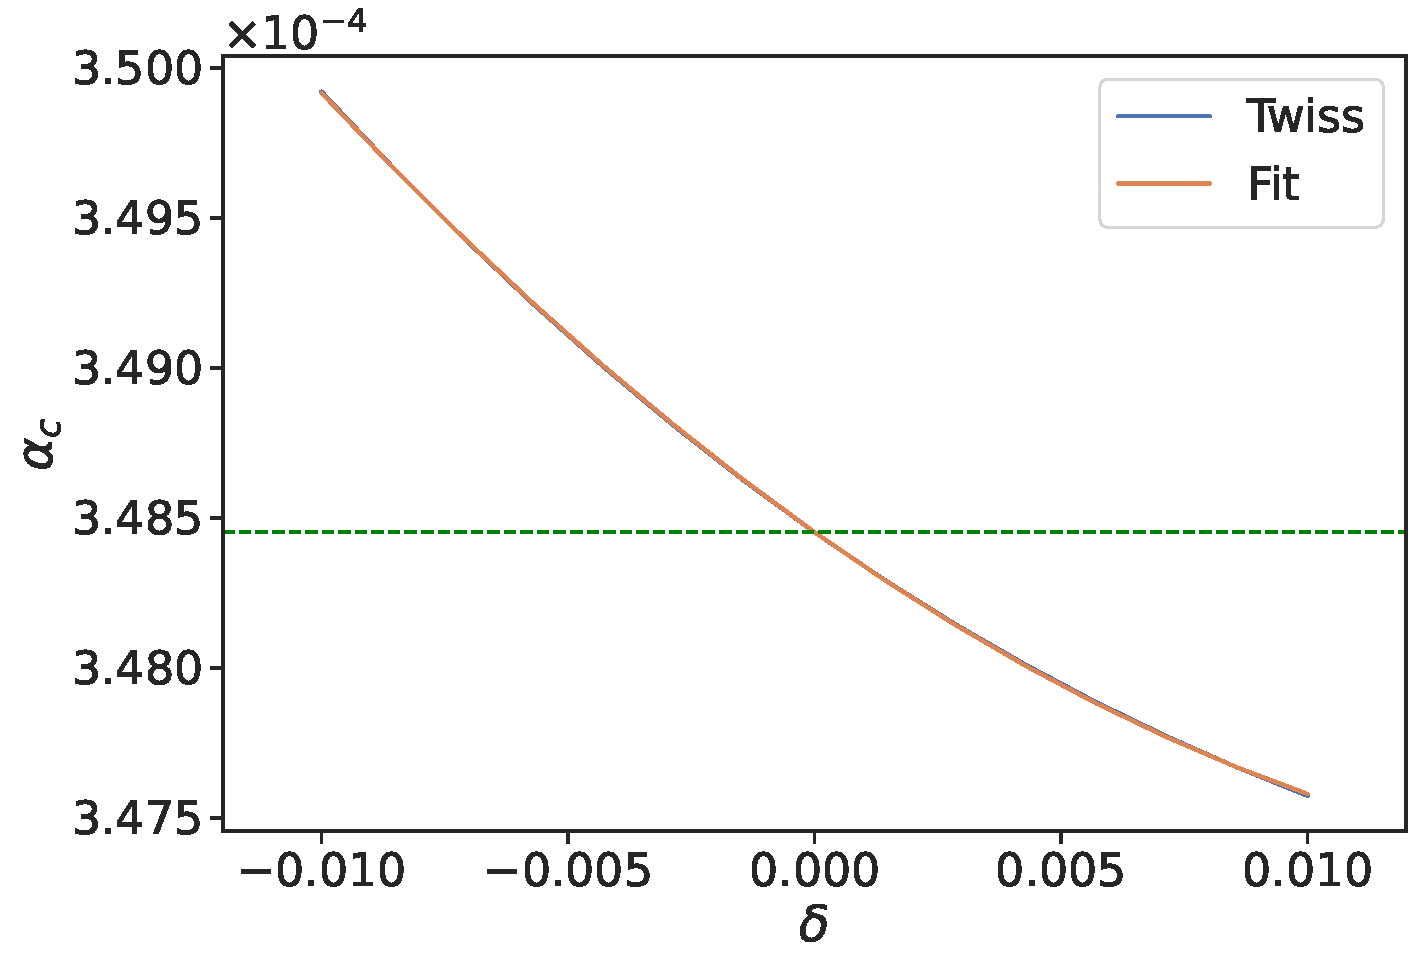
\includegraphics[width=\textwidth]{images/higher_order_momentum_compaction_factor.pdf}
        \caption{Non-linear fit of $\alpha_c$ obtained via an evaluation at discrete $\delta$ in
        MAD-X. The green line represents a constant $\alpha_c = \alpha_{c,0}$.}
    \end{subfigure}
    \hfill
    \begin{subfigure}[t]{0.48\textwidth}
        \centering
        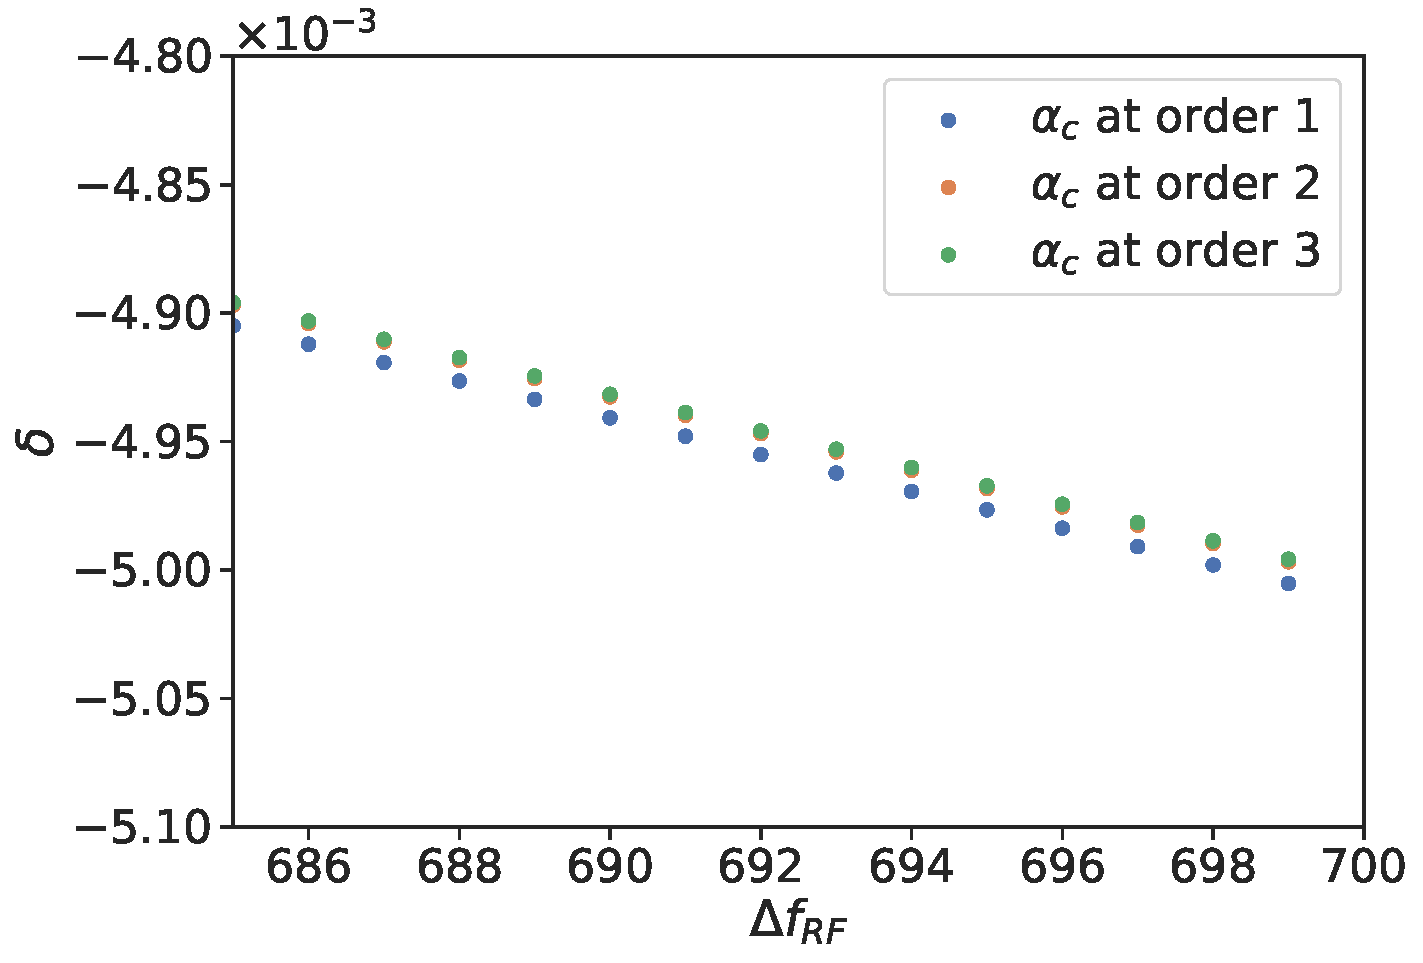
\includegraphics[width=\textwidth]{images/delta_vs_frf_alpha_c.pdf}
        \caption{Divergence of the momentum offset when considering higher $\alpha_c$ orders with
        large RF trims.}
    \end{subfigure}
    \caption{Non linearity of $\alpha_c$ and its effect on the computed $\delta$ via RF trims. The
    simulations are done at injection energy of 450 GeV.}
    \label{fig:decapoles:chromaticity:momentum_compaction_factor}
\end{figure}

It is observed that while clearly depending on higher orders, the momentum compaction factor only
has a small impact on the calculated $\delta$.
\Cref{fig:decapoles:chromaticity:momentum_compaction_factor_chroma_meas} shows a real-life 
measurement, comparing the fit of the chromaticity function with various $\delta$, computed up to
the third order of $\alpha_c$.

\begin{figure}[!htb]
    \centering
    \begin{subfigure}[t]{0.48\textwidth}
        \centering
        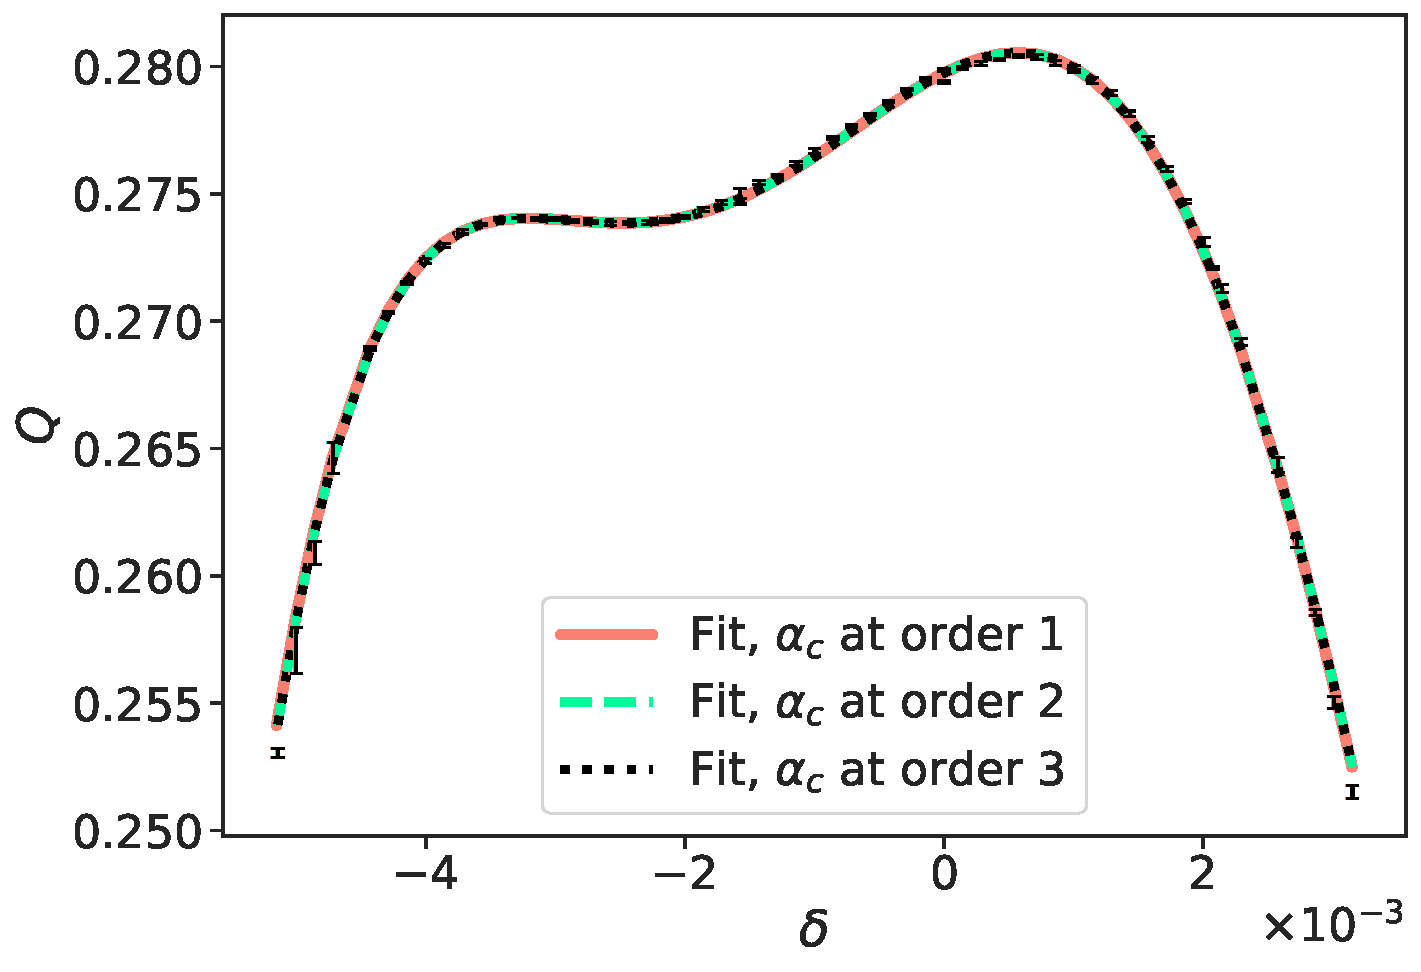
\includegraphics[width=\textwidth]{images/chroma_function_alpha_c.pdf}
        \caption{Fit of the chromaticity function at the $5^{\text{th}}$ order, considering the
        $\alpha_c$ expansion up to the third order.}
    \end{subfigure}
    \hfill
    \begin{subfigure}[t]{0.48\textwidth}
        \centering
        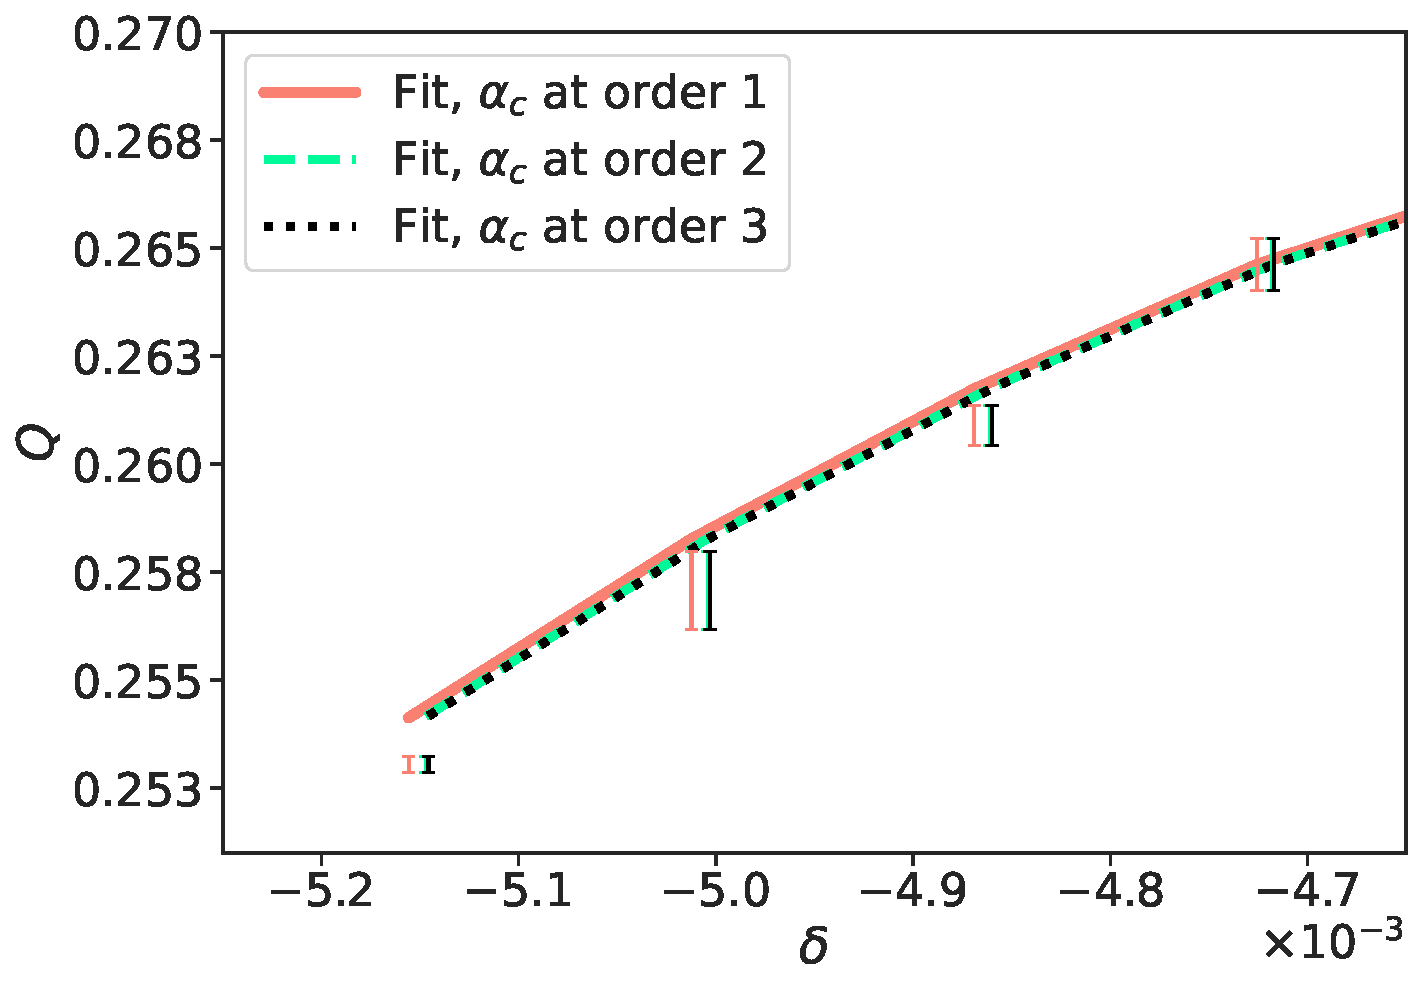
\includegraphics[width=\textwidth]{images/chroma_function_alpha_c_zoom.pdf}
        \caption{Zoom on one side of the fit. The difference between the second and third order
        is barely noticeable.}
    \end{subfigure}
    \caption{Fit of the chromaticity function considering several $\alpha_c$ orders.}
    \label{fig:decapoles:chromaticity:momentum_compaction_factor_chroma_meas}
\end{figure}

The fit of the chromaticity function is barely impacted when considering the higher orders of the 
momentum compaction factor. The different orders of the chromaticity are collected
in~\cref{table:decapoles:chromaticity:alpha_c_chroma}.
The higher order terms of $\alpha_c$ can thus be neglected and are not a source of higher
chromaticity orders.

\begin{table}[!htb]
    \centering
    \begin{tabular}{lrrr}
      \toprule
                  & \multicolumn{3}{c}{$\alpha_c$ order} \\
  %                \cmidrule{2-4}
      Chromaticity &  \multicolumn{1}{c}{1}  &  \multicolumn{1}{c}{2} &  \multicolumn{1}{c}{3} \\
      \midrule
      $Q^{(1)}$ & $ 2.52 \pm 0.03$ & $ 2.53 \pm 0.03$ & $ 2.53 \pm 0.03$ \\
      $Q^{(2)}$ & $-3.04 \pm 0.05$ & $-3.05 \pm 0.05$ & $-3.05 \pm 0.05$ \\
      $Q^{(3)}$ & $-4.75 \pm 0.03$ & $-4.75 \pm 0.03$ & $-4.75 \pm 0.03$ \\
      $Q^{(4)}$ & $-0.33 \pm 0.07$ & $-0.32 \pm 0.07$ & $-0.32 \pm 0.07$ \\
      $Q^{(5)}$ & $ 2.33 \pm 0.06$ & $ 2.36 \pm 0.06$ & $ 2.36 \pm 0.06$ \\
      \bottomrule
    \end{tabular}
    \caption{Chromaticity values obtained for the same measurement, depending on the order of the
    momentum compaction factor taken into account.}
    \label{table:decapoles:chromaticity:alpha_c_chroma}
\end{table}     



%----------------------------------------
%             Noisy Tune
\FloatBarrier
\subsubsection{\review{Noise and Spectral Lines}}

Noise lines from the electronics can be observed in the raw data obtained from the BBQ tune system.
Occasionally, when these are strong, their frequency peaks can be mistaken for the actual
tune and subsequently logged by the system. This leads to significant uncertainties in the
measurement, especially when these data points cannot be reliably classified as outliers. An example
of a tune measurement affected by this issue is shown in
\cref{fig:decapoles:chromaticity:noisy_tune}. However, this incorrect tune identification was not
problematic for measurements with narrower momentum offset ranges, as the induced tune shift was
smaller and therefore the tune less likely to overlap with strong noise lines.

\begin{figure}[!htb]
    \centering
    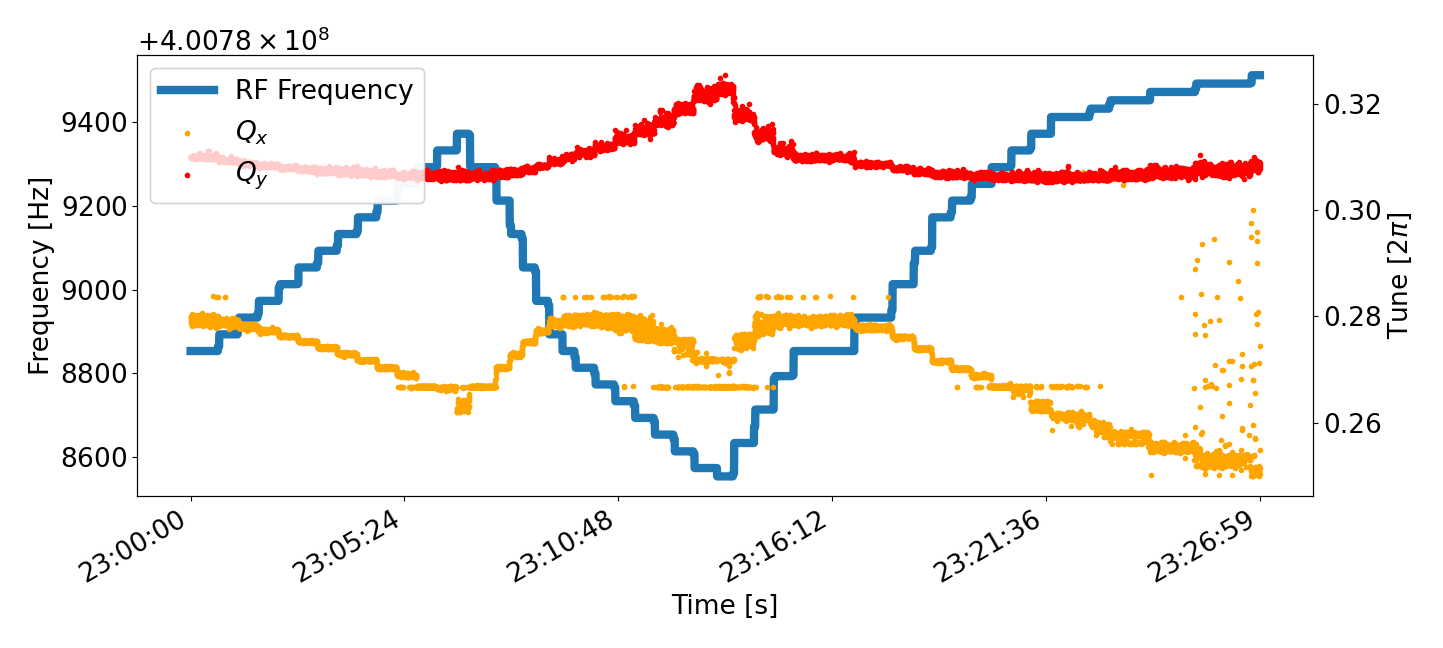
\includegraphics[width=\textwidth]{./images/noisy_tune.png}
    \caption{Shift of the tune by variation of the RF. Noise lines can appear in some cases,
    making the tune error-bar large or downright unusable.}
    \label{fig:decapoles:chromaticity:noisy_tune}
\end{figure}

A solution to this issue is to use the raw data extracted from the BBQ system. From there, a
spectrogram clearly shows the noise lines, as seen in \cref{fig:decapoles:chromaticity:spectrogram}.
Those lines have been repeatedly identified over several measurements and confirmed to be static.
The highest peak in the spectrogram can be reliably identified by removing unwanted lines,
resulting in a cleaner measurement. It is also important to note that the BBQ system requires the
tune window to be set, which, if overlooked, can lead to erroneous data. By analyzing the raw data,
it is ensured that correct data is used, preventing the measurement from inadvertently capturing
noise.

\begin{figure}[!htb]
    \centering
    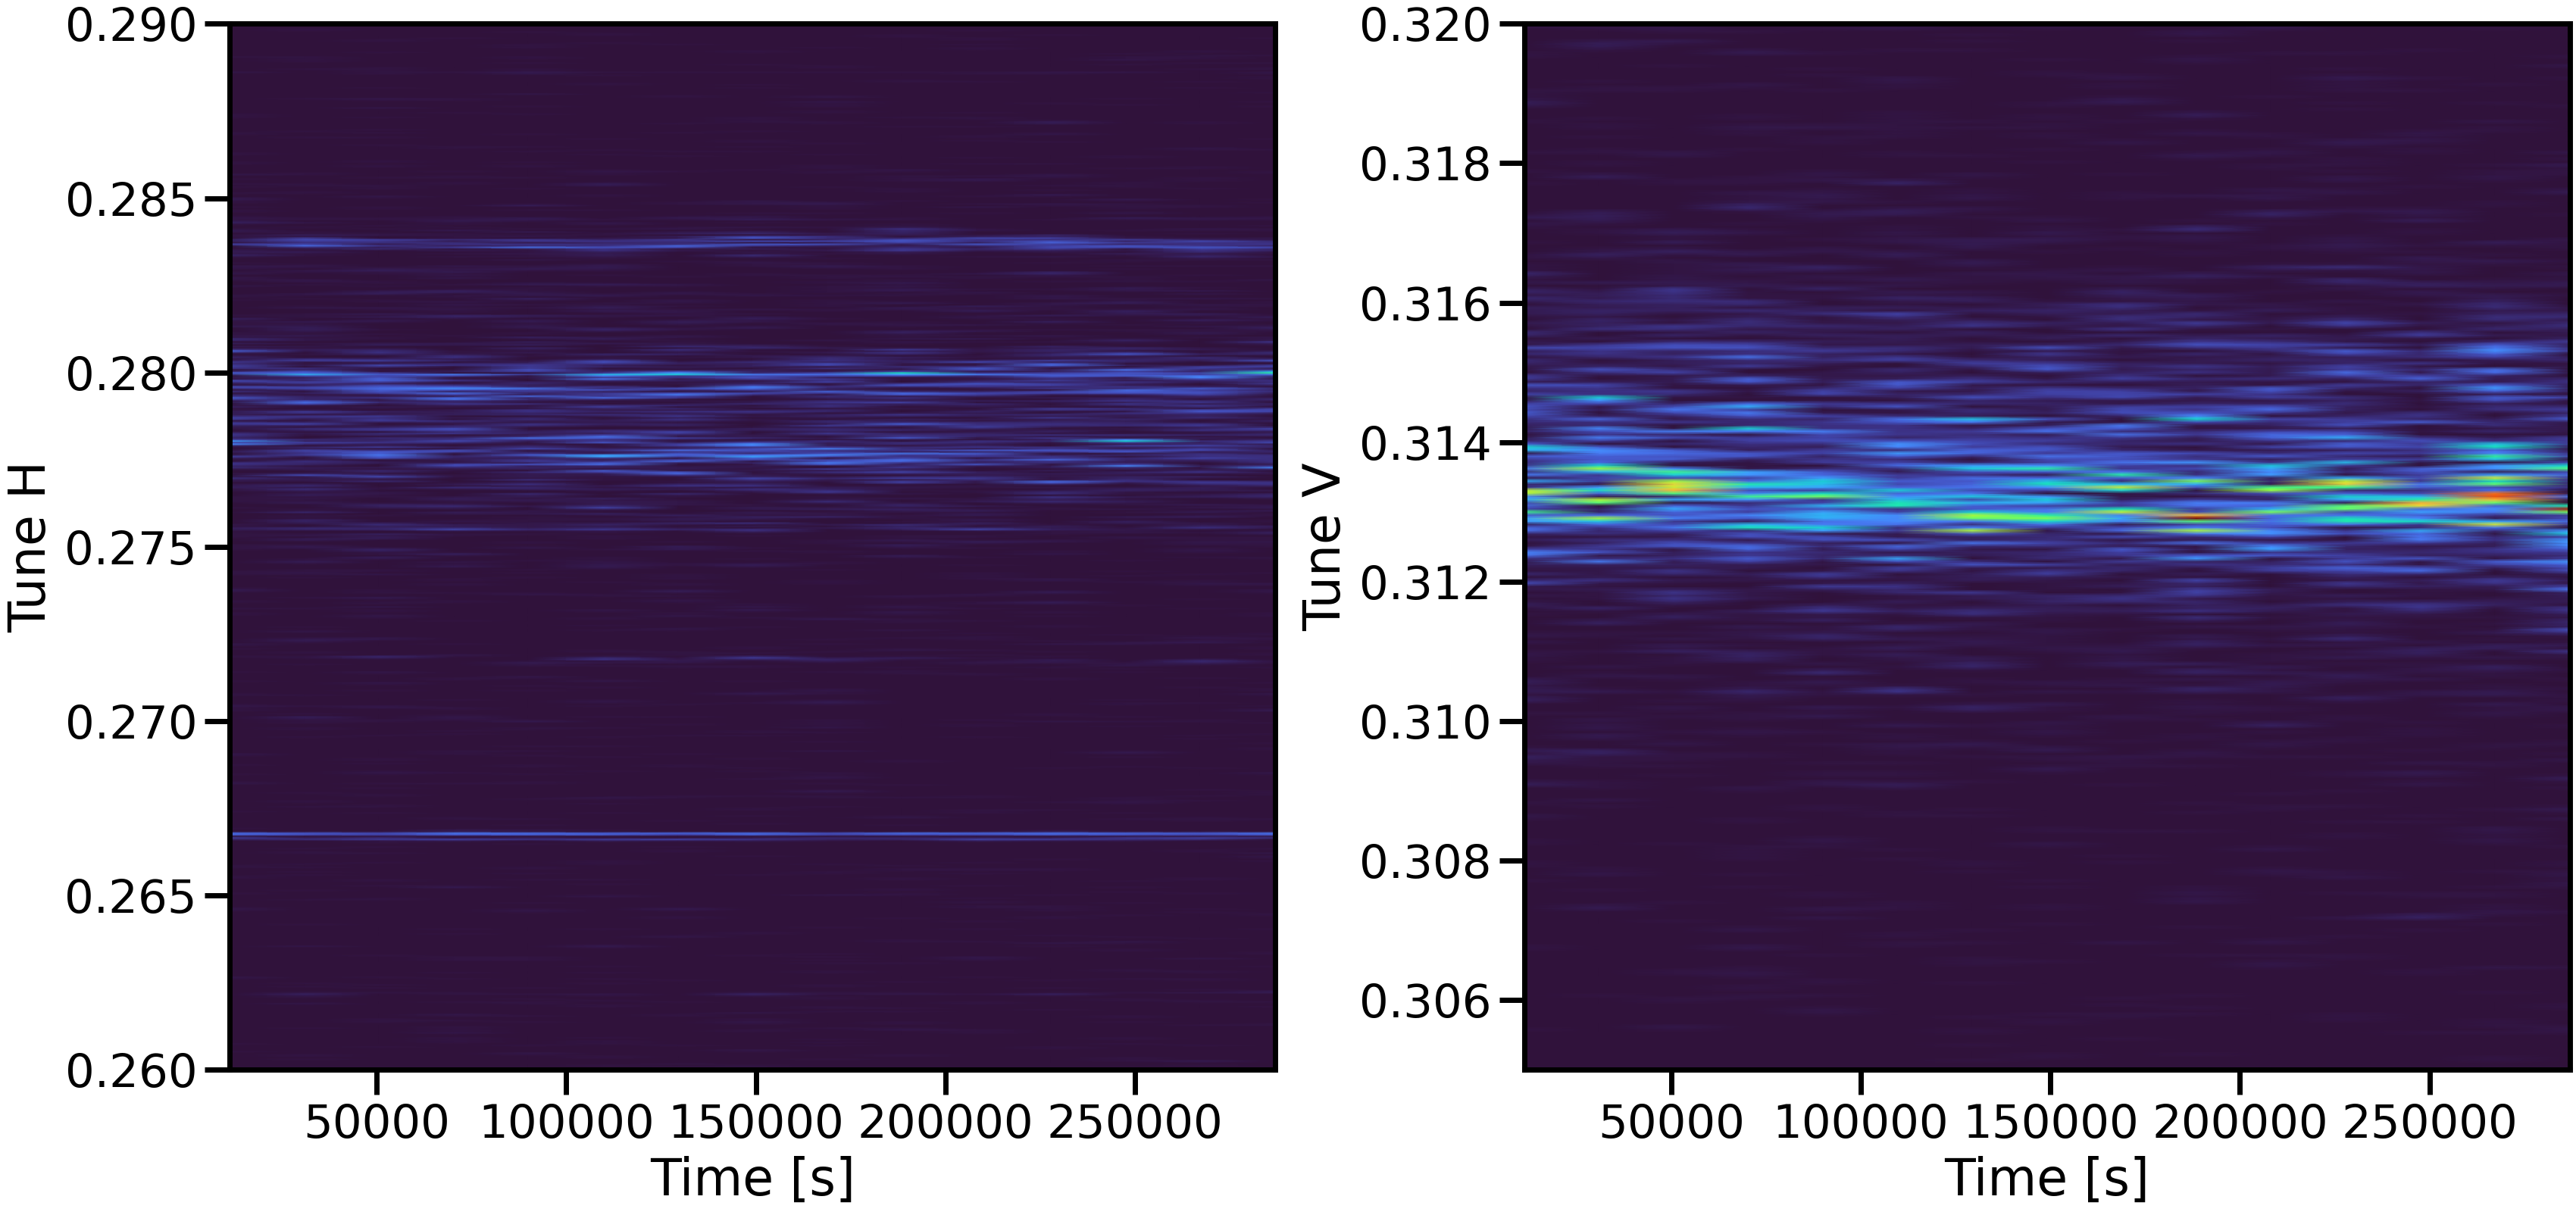
\includegraphics[width=.8\textwidth]{./images/spectrogram.png}
    \caption{Tune spectrogram obtained via the BBQ system. Strong noise lines can be seen above and
    below where the tune really is, causing the wrong frequency peak to be identified as the tune.
    These lines are always observed around $Q = 0.266$ and $Q = 0.284$}
    \label{fig:decapoles:chromaticity:spectrogram}
\end{figure}




%----------------------------------------
%         Other dpp Measurements
\FloatBarrier
\subsubsection{\review{Momentum Offset from Orbit}}

The momentum offset $\delta$ can be reconstructed through several methods. One such method,
based on beams's orbit, was previously stored by the LHC's logging services but is not
anymore. Reconstructing the momentum offset can introduce uncertainties due to the
non-linearities of both the momentum compaction factor, as discussed earlier, and the dispersion.

To evaluate this, a re-analysis of previous Run~2 measurements was conducted using the RF formula,
with the goal of comparing the resulting non-linear chromaticity values.
\Cref{fig:very_high_orders:bare_chroma_2016} shows the chromaticity measurements for Beam 1 and Beam
2 in both planes, with chromaticity computed via both the orbit-based and RF-based methods. A
numerical comparison is provided in \cref{table:very_high_orders:bare_chroma_2016}.

The lack of discrepancy between the two techniques suggests that the measurements were operating
within the linear regime of the dispersion and momentum compaction factor, and no detuning effects
were present that could have been misinterpreted as a higher-order chromaticity.

\begin{table}[!htb]
    \centering
    \begin{tabular}{lrrrr}
        \toprule
              & \multicolumn{2}{c}{$\delta$ via RF}  &  \multicolumn{2}{c}{$\delta$ via orbit} \\
        Plane & \multicolumn{1}{c}{$Q'' [10^3]$}     & \multicolumn{1}{c}{$Q''' [10^6]$} & \multicolumn{1}{c}{$Q'' [10^3]$} & \multicolumn{1}{c}{$Q''' [10^6]$}\\
        \midrule
        Beam 1 &&&& \\
        \hspace{2mm}X & $-0.64 \pm 0.01$ & $ 3.00 \pm 0.04$   & $-0.62 \pm 0.01$ & $ 2.91 \pm 0.04$ \\
        \hspace{2mm}Y & $-0.17 \pm 0.01$ & $-2.12 \pm 0.04$   & $-0.14 \pm 0.01$ & $-2.09 \pm 0.04$ \\
        Beam 2 &&&& \\
        \hspace{2mm}X & $-1.18 \pm 0.02$ & $ 2.89 \pm 0.06$   & $-1.23 \pm 0.03$ & $ 3.13 \pm 0.11$ \\
        \hspace{2mm}Y & $ 0.18 \pm 0.02$ & $-1.95 \pm 0.05$   & $ 0.20 \pm 0.02$ & $-2.02 \pm 0.06$ \\
        \bottomrule
    \end{tabular}
    \caption{Comparison of the chromaticity values obtained for the same measurement via two
    different methods to acquire $\delta$.}
    \label{table:very_high_orders:bare_chroma_2016}
  \end{table}


\begin{figure}[!htb]
    \begin{subfigure}{0.49\textwidth}
        \centering
        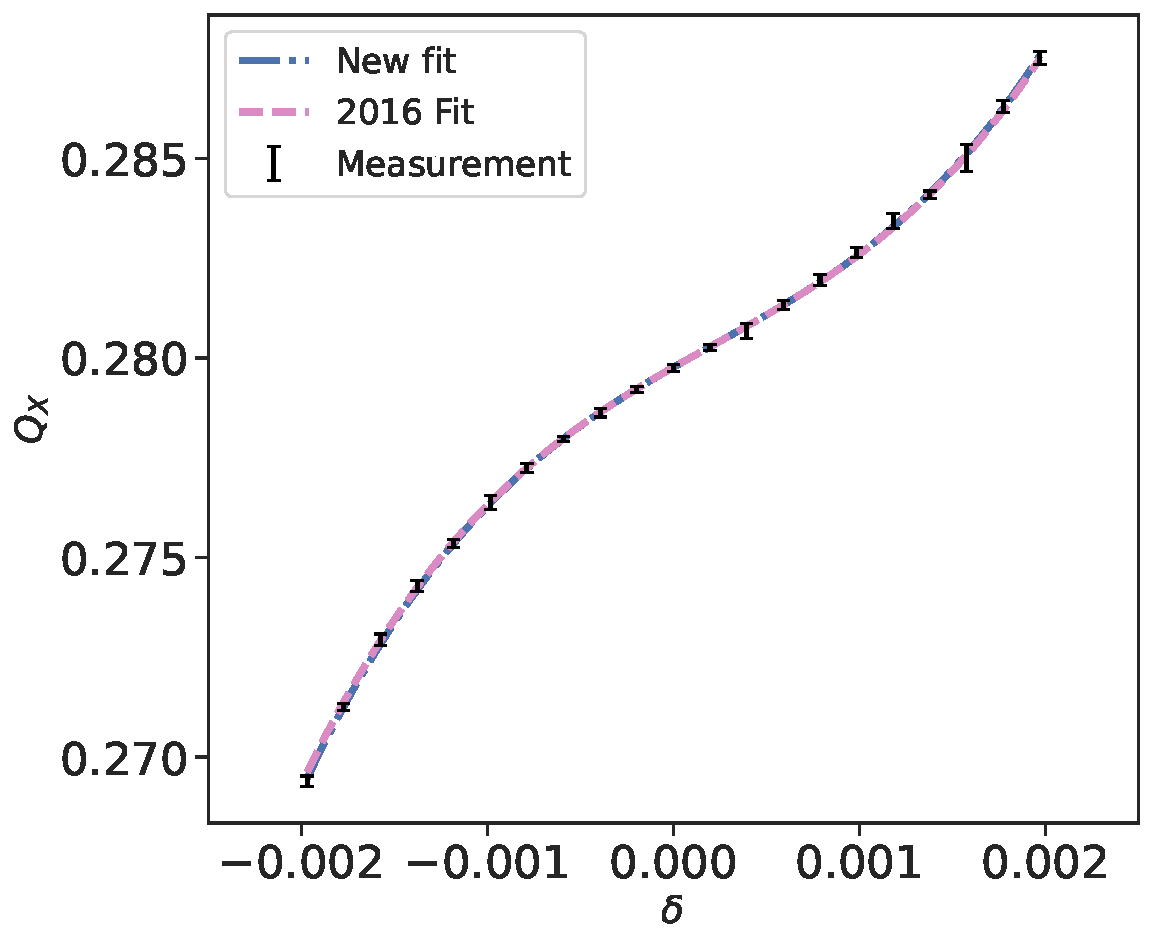
\includegraphics[width=\textwidth]{./images/chromaticity_2016/B1_qx.pdf}
        \caption{$Q_x$ Beam 1}
    \end{subfigure}
    \hfill
    \begin{subfigure}{0.49\textwidth}
        \centering
        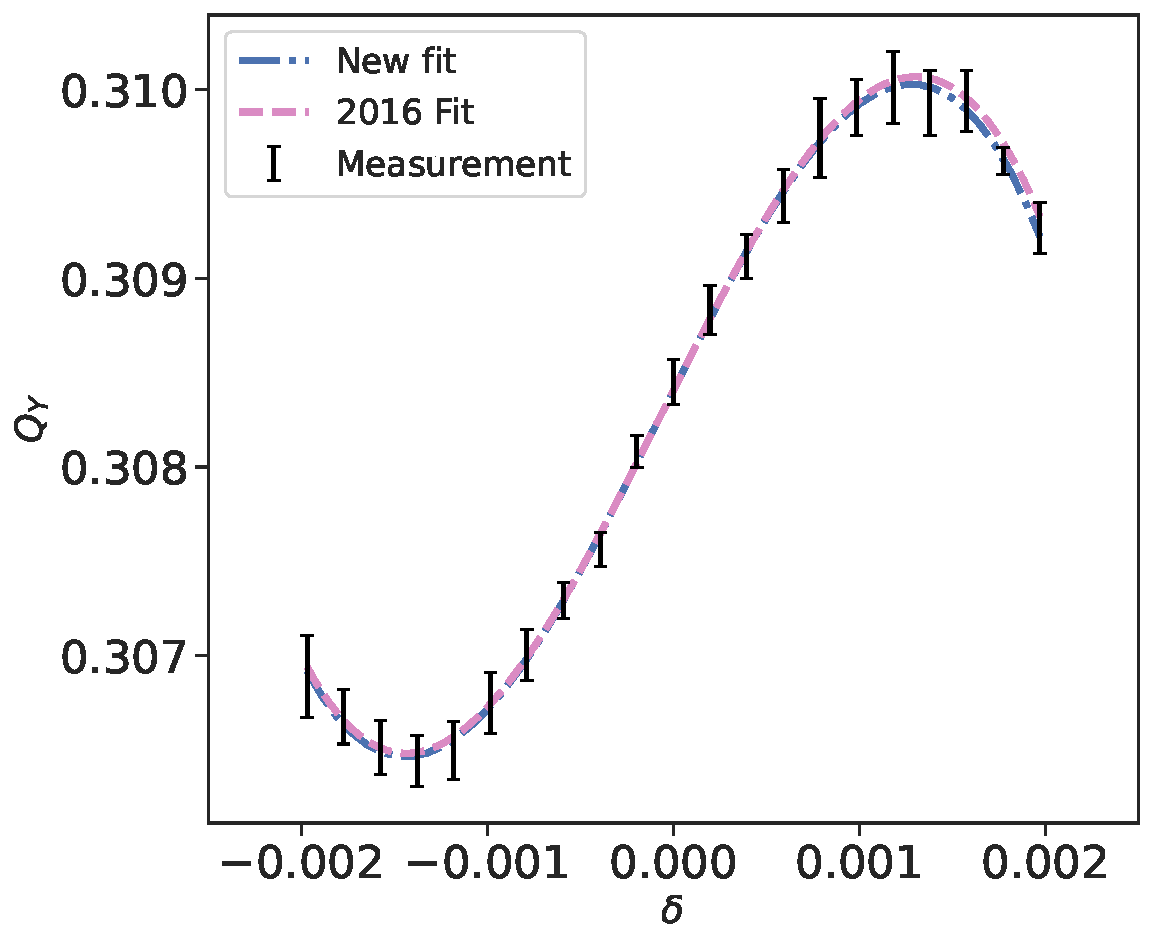
\includegraphics[width=\textwidth]{./images/chromaticity_2016/B1_qy.pdf}
        \caption{$Q_y$ Beam 1}
    \end{subfigure}
    %
    \\
    %
    \begin{subfigure}{0.49\textwidth}
        \centering
        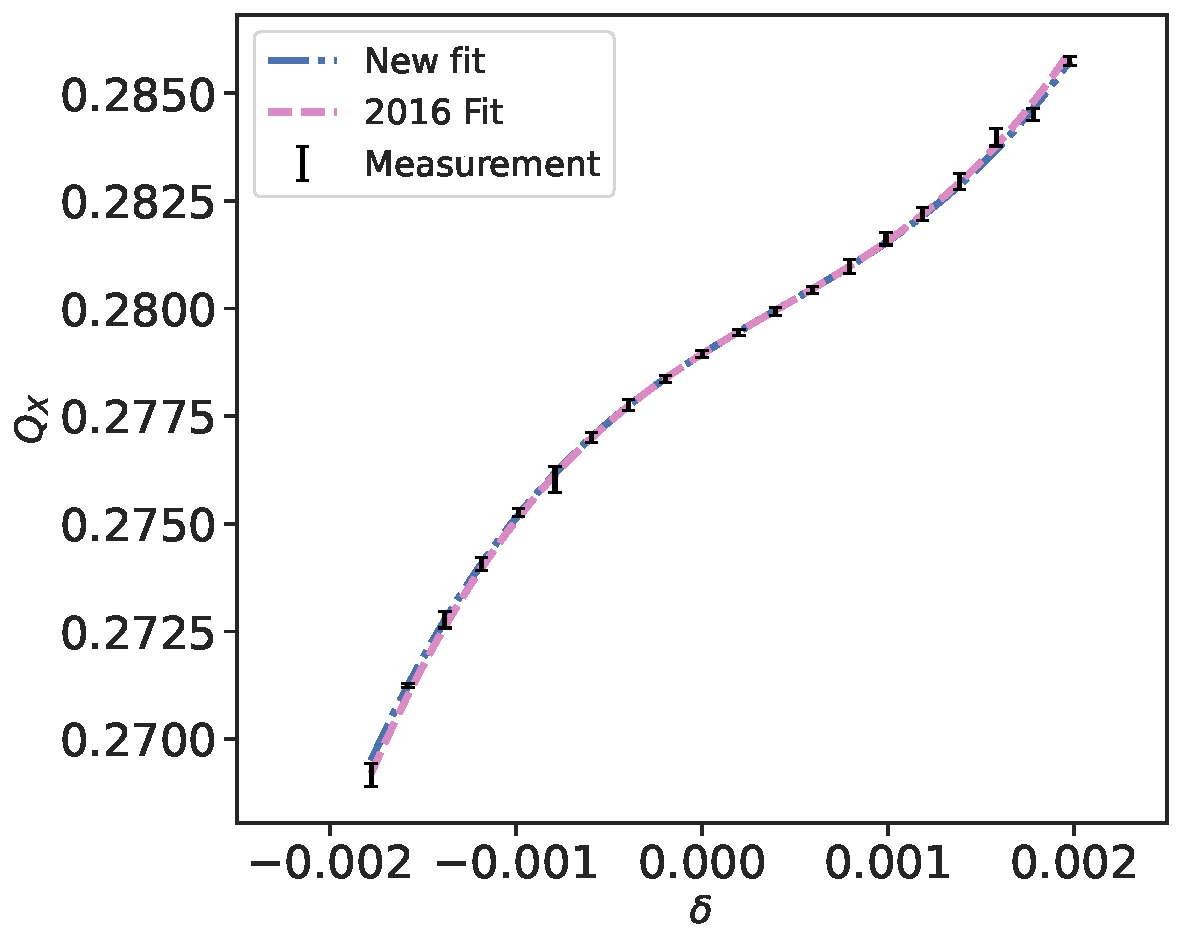
\includegraphics[width=\textwidth]{./images/chromaticity_2016/B2_qx.pdf}
        \caption{$Q_x$ Beam 2}
    \end{subfigure}
    \hfill
    \begin{subfigure}{0.49\textwidth}
        \centering
        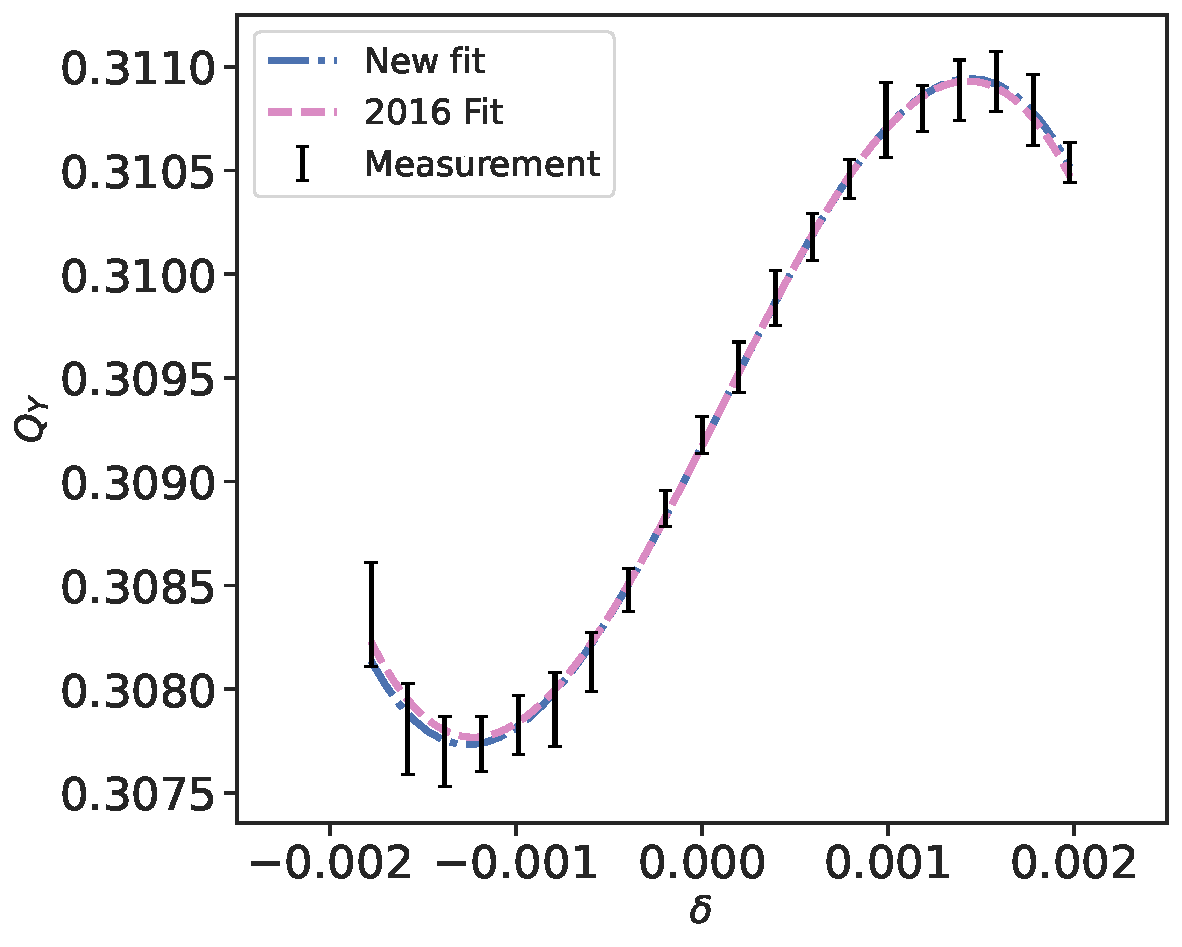
\includegraphics[width=\textwidth]{./images/chromaticity_2016/B2_qy.pdf}
        \caption{$Q_y$ Beam 2}
    \end{subfigure}
    \caption{Comparison of the non-linear chromaticity fit obtained from the computed momentum
    offset via the RF in 2022 and from the logged values in 2016.}
    \label{fig:very_high_orders:bare_chroma_2016}
\end{figure}



\FloatBarrier
%----------------------------------------
%      Other Performed Measurements
%----------------------------------------
\subsection{\review{Further Measurements}}

In order to assess the correctness of the observation of higher chromaticity orders, measurement
repeatability is needed. Two measurements were thus taken in 2022, with different configurations
pertaining to the correction of the second and third order chromaticities $Q''$ and $Q'''$. 
The first one used the nominal correction strengths for octupole and decapole corrector magnets,
derived from magnetic measurements, where the second one used beam-based corrections for the same
elements, computed from the previous measurement.
More measurements were taken during 2024's commissioning with new optics for the same reasons, to
minimize the second and third order chromaticities. Three measurements were taken: with nominal
corrections, after having corrected $Q'''$  and then $Q''$. The introduced new optics mainly changed
the powering of the triplets at the IPs and are not expected to have a considerable impact on the
chromaticity. 

\Cref{table:high_orders:dpp_ranges} shows a summary of those measurements with their respective 
achieved momentum offset ranges. While the 2024 measurements achieved greater ranges than the
previous ones, those were restricted during analysis to allow suitable comparisons.

\begin{table}[!htb]
  \centering
  \begin{tabular}{lllcc}
    \toprule
    Number & Year & Corrections      & $\delta$ min. $[\times 10^{-3}]$ & $\delta$ max. $[\times 10^{-3}]$  \\
    \midrule
    1 & 2022 & Nominal          & $-3.15$ & $3.01$  \\
    2 & 2022 & $Q''$ \& $Q'''$  & $-3.15$ & $3.72$  \\
    3 & 2024 & Nominal          & $-5.15$ & $3.15$  \\
    4 & 2024 & $Q'''$           & $-3.44$ & $4.87$  \\
    5 & 2024 & $Q''$ \& $Q'''$  & $-3.86$ & $4.44$  \\
    \bottomrule
  \end{tabular}
  \caption{Performed chromaticity measurements with their respective momentum offset ranges.}
  \label{table:high_orders:dpp_ranges}
\end{table}

In order to stay consistent, the horizontal and vertical tunes were respectively set to $Q_x = 0.28$
and $Q_y = 0.31$ for all measurements. The linear chromaticity $Q'$ is set to a small value, around
$2$, to avoid large tune shifts throughout the scan.
All measurements were performed during LHC's beam commissioning.
%, as part of the measurements and corrections performed after technical or long shutdowns.



%--------------------------------------
%       Varying Configurations
\subsubsection{\review{Varying Configurations}}

The five previously introduced measurements were performed with very different configurations for
the octupolar and decapolar correctors. \Cref{tab:high_orders:mcdo_values_corr} shows the strengths
applied on every circuit for each correction scheme, in 2022. The correction is called 
\textit{global} as all correctors are trimmed uniformly. The 2024 corrections are similar in order
of magnitude.
\Cref{fig:high_orders:comparison_2022_2024} shows the measurements and fit of some of these
measurements, to highlight their differences.

\begin{table}[H]
  \centering
  \begin{tabular}{lll}
  \toprule
    Beam  &    $K_4 [\mathrm{m}^{-4}]$      &  $K_5 [\mathrm{m}^{-5}]$  \\
  \midrule
      1   &   +3.2973    &  +1610   \\
      2   &   +2.1716    &  +1618   \\
  \bottomrule
  \end{tabular}
  \caption{Corrections applied on top of the nominal octupolar and decapolar correctors strengths in
  2022 for the $Q''$ and $Q'''$ corrections.}
  \label{tab:high_orders:mcdo_values_corr}
\end{table}

\begin{figure}[H]
  \centering
  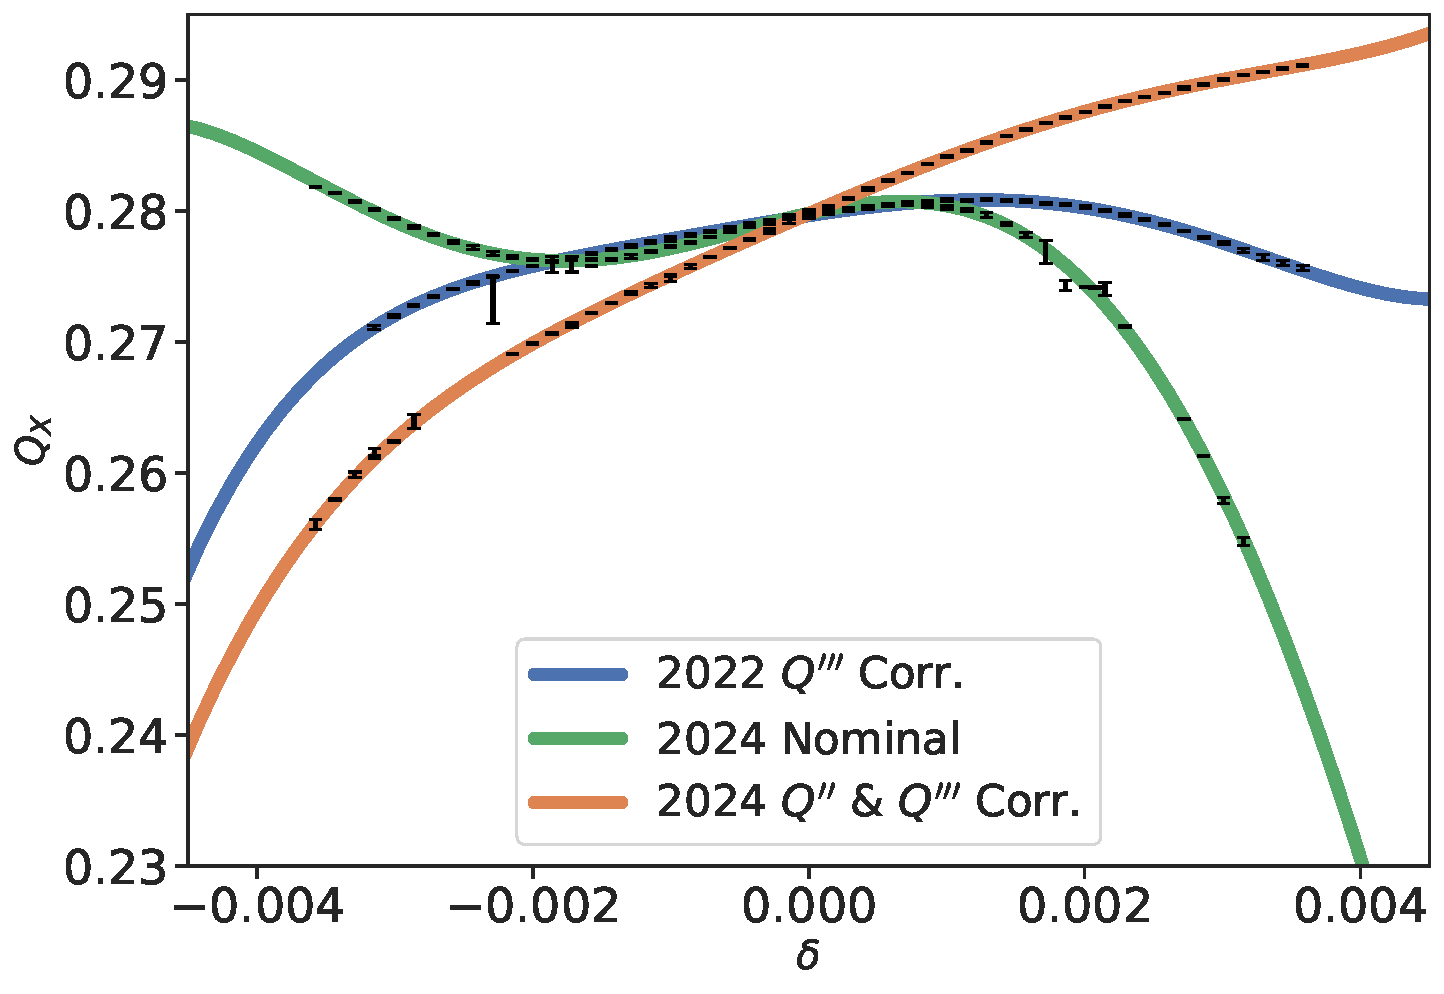
\includegraphics[width=0.7\textwidth]{./images/chromaticity_2024_vs_2022/chroma_comparison_B1_X.pdf}
  \caption{Selection of horizontal chromaticity measurements performed with varying configurations
  of the octupolar and decapolar correctors for Beam 1 during the commissionings of 2022 and 2024.}
  \label{fig:high_orders:comparison_2022_2024}
\end{figure}

A summary of the measured chromaticity orders is given in \cref{fig:high_oders:all_values}.  
The first measurement in the horizontal plane of Beam 2 suffered from low beam intensity and worse
noise, resulting in a high correlation between $Q^{(4)}$ and $Q^{(5)}$, and is therefore not included. The
last measurement for the vertical plane experienced some tune drift, making the fit impossible and
is therefore not included for both beams.

% The average is weighted by the errors
\begin{table}
  \centering
  \small
  \begin{tabular}{lrrrrr}
    \toprule
    Axis & Meas. & $Q''$ & $Q'''$ & $Q^{(4)}$ & $Q^{(5)}$ \\
    \midrule
    Horizontal &&&&&\\
    \hspace{2mm}Beam 1 & 1 & $-2.44\pm0.02$ & $-3.37\pm0.04$ & $-0.56\pm0.02$ & $ 1.21\pm0.07$ \\
                       & 2 & $-0.61\pm0.01$ & $-1.00\pm0.03$ & $-0.62\pm0.02$ & $ 1.19\pm0.05$ \\
                       & 3 & $-2.01\pm0.05$ & $-4.49\pm0.10$ & $-0.58\pm0.07$ & $ 1.34\pm0.18$ \\
                       & 4 & $-1.46\pm0.03$ & $-0.29\pm0.06$ & $-0.43\pm0.04$ & $ 1.09\pm0.10$ \\
                       & 5 & $-0.33\pm0.01$ & $-0.31\pm0.03$ & $-0.59\pm0.01$ & $ 0.75\pm0.04$ \\
                       & \textbf{Avg.}&     &                & $-0.56\pm0.07$ & $ 1.12\pm0.20$ \\%[0.5em]
                       \hdashline\noalign{\vskip 1ex}
    \hspace{2mm}Beam 2% & 1 & $-2.45\pm0.03$ & $-2.72\pm0.08$ & $-1.00\pm0.05$ & $ 0.15\pm0.14$ \\  % bad correlation for n°1
                       & 2 & $-0.85\pm0.01$ & $-0.66\pm0.03$ & $-0.57\pm0.02$ & $ 1.09\pm0.06$ \\
                       & 3 & $-2.93\pm0.05$ & $-4.40\pm0.08$ & $-0.53\pm0.08$ & $ 1.66\pm0.16$ \\
                       & 4 & $-2.21\pm0.02$ & $-0.00\pm0.03$ & $-0.46\pm0.02$ & $ 1.18\pm0.05$ \\
                       & 5 & $-0.53\pm0.02$ & $-0.09\pm0.03$ & $-0.57\pm0.02$ & $ 0.98\pm0.05$ \\
                       & \textbf{Avg.}&     &                & $-0.53\pm0.04$ & $ 1.23\pm0.26$ \\%[0.5em]
                       \midrule
    Vertical &&&&&\\
    \hspace{2mm}Beam 1 & 1 & $ 0.97\pm0.02$ & $ 1.62\pm0.05$ & $ 0.15\pm0.03$ & $-0.88\pm0.09$ \\
                       & 2 & $-0.23\pm0.01$ & $ 0.13\pm0.02$ & $ 0.09\pm0.02$ & $-0.60\pm0.03$ \\
                       & 3 & $ 0.83\pm0.02$ & $ 1.97\pm0.03$ & $ 0.29\pm0.02$ & $-0.68\pm0.05$ \\
                       & 4 & $ 0.62\pm0.01$ & $-0.18\pm0.03$ & $ 0.00\pm0.02$ & $-0.56\pm0.05$ \\
                       %& 5 & $-0.28\pm0.02$ & $-0.25\pm0.04$ & $ 0.28\pm0.02$ & $-0.12\pm0.05$ \\
                       & \textbf{Avg.}&     &                & $ 0.13\pm0.11$ & $-0.68\pm0.12$ \\%[0.5em]
                       \hdashline\noalign{\vskip 1ex}
    \hspace{2mm}Beam 2 & 1 & $ 0.79\pm0.03$ & $ 1.54\pm0.06$ & $ 0.24\pm0.04$ & $-0.74\pm0.13$ \\
                       & 2 & $-0.29\pm0.01$ & $ 0.10\pm0.02$ & $ 0.13\pm0.02$ & $-0.58\pm0.04$ \\
                       & 3 & $ 0.89\pm0.02$ & $ 2.05\pm0.03$ & $ 0.32\pm0.03$ & $-0.73\pm0.06$ \\
                       & 4 & $ 0.60\pm0.02$ & $-0.14\pm0.03$ & $ 0.04\pm0.02$ & $-0.66\pm0.05$ \\
                       %& 5 & $-0.62\pm0.02$ & $-0.29\pm0.04$ & $ 0.29\pm0.02$ & $-0.19\pm0.06$ \\
                       & \textbf{Avg.}&     &                & $ 0.18\pm0.11$ & $-0.68\pm0.06$ \\%[0.5em]
    \bottomrule
  \end{tabular}
  \caption{Summary of the chromaticity values obtained from the measurements presented in
  \cref{table:high_orders:dpp_ranges}.}
  \label{fig:high_oders:all_values}
\end{table}

The consistent identification of fourth and fifth order chromaticity across various configurations
of the LHC, with differing lower order chromaticity and coupling, enhances confidence in their
identification. Previous studies have typically focused on fits limited to the third order. However,
expanding the analysis to include fifth order not only increases the estimate of $Q'''$ but also
enhances the overall fit quality. Accurately measuring third order chromaticity is crucial for its
correction, underscoring the importance of considering higher order terms.


\FloatBarrier
%----------------------------------------
%            Model Estimates
%----------------------------------------
\subsection{\review{Model Estimates}}
\label{sec:nl_chroma_model}

Benchmarking the magnetic model of the LHC is important, in order to gauge its correctness and that
of the error tables in use, and address any potential discrepancies. The model of the LHC is based on
MADX and magnetic field error tables~\cite{p_hagen_wise_2006}, containing seeds for the random
errors. To compute the chromaticity, simulations are run via PTC, with a selection of these field 
errors.

Simulations incorporating various field errors have been conducted to evaluate the contributions of
individual magnet orders to fourth and fifth order chromaticity. Field errors
are applied to all magnets, with $b_2$ errors in the main dipoles resulting in a $\beta$-beating of
approximately $10\%$. Coupling is introduced using global knobs to create a $C^-$ value of $0.001$,
which is commonly observed during operation. Normal and skew field errors, ranging from sextupolar
($b_3$) to decahexapolar ($b_8$), are added either individually or in combination to determine which
has the strongest effect.


% ----------------------------------
\paragraph{\review{Fourth Order Chromaticity}}

The results from simulations strongly imply that the dodecapolar errors are the main contributors
to $Q^{(4)}$, as can be seen in \cref{fig:high_orders:beam1_q4_ptc}.
The most notable effect on this chromaticity order is the beta-beating, introducing a very large
spread via the various error seeds.
Comparing the simulation at the top with most errors added, the $b_6$ component alone accounts for
$\approx 70\%$ of it for both axes on each beam.

\begin{figure}[!htb]
    \centering
    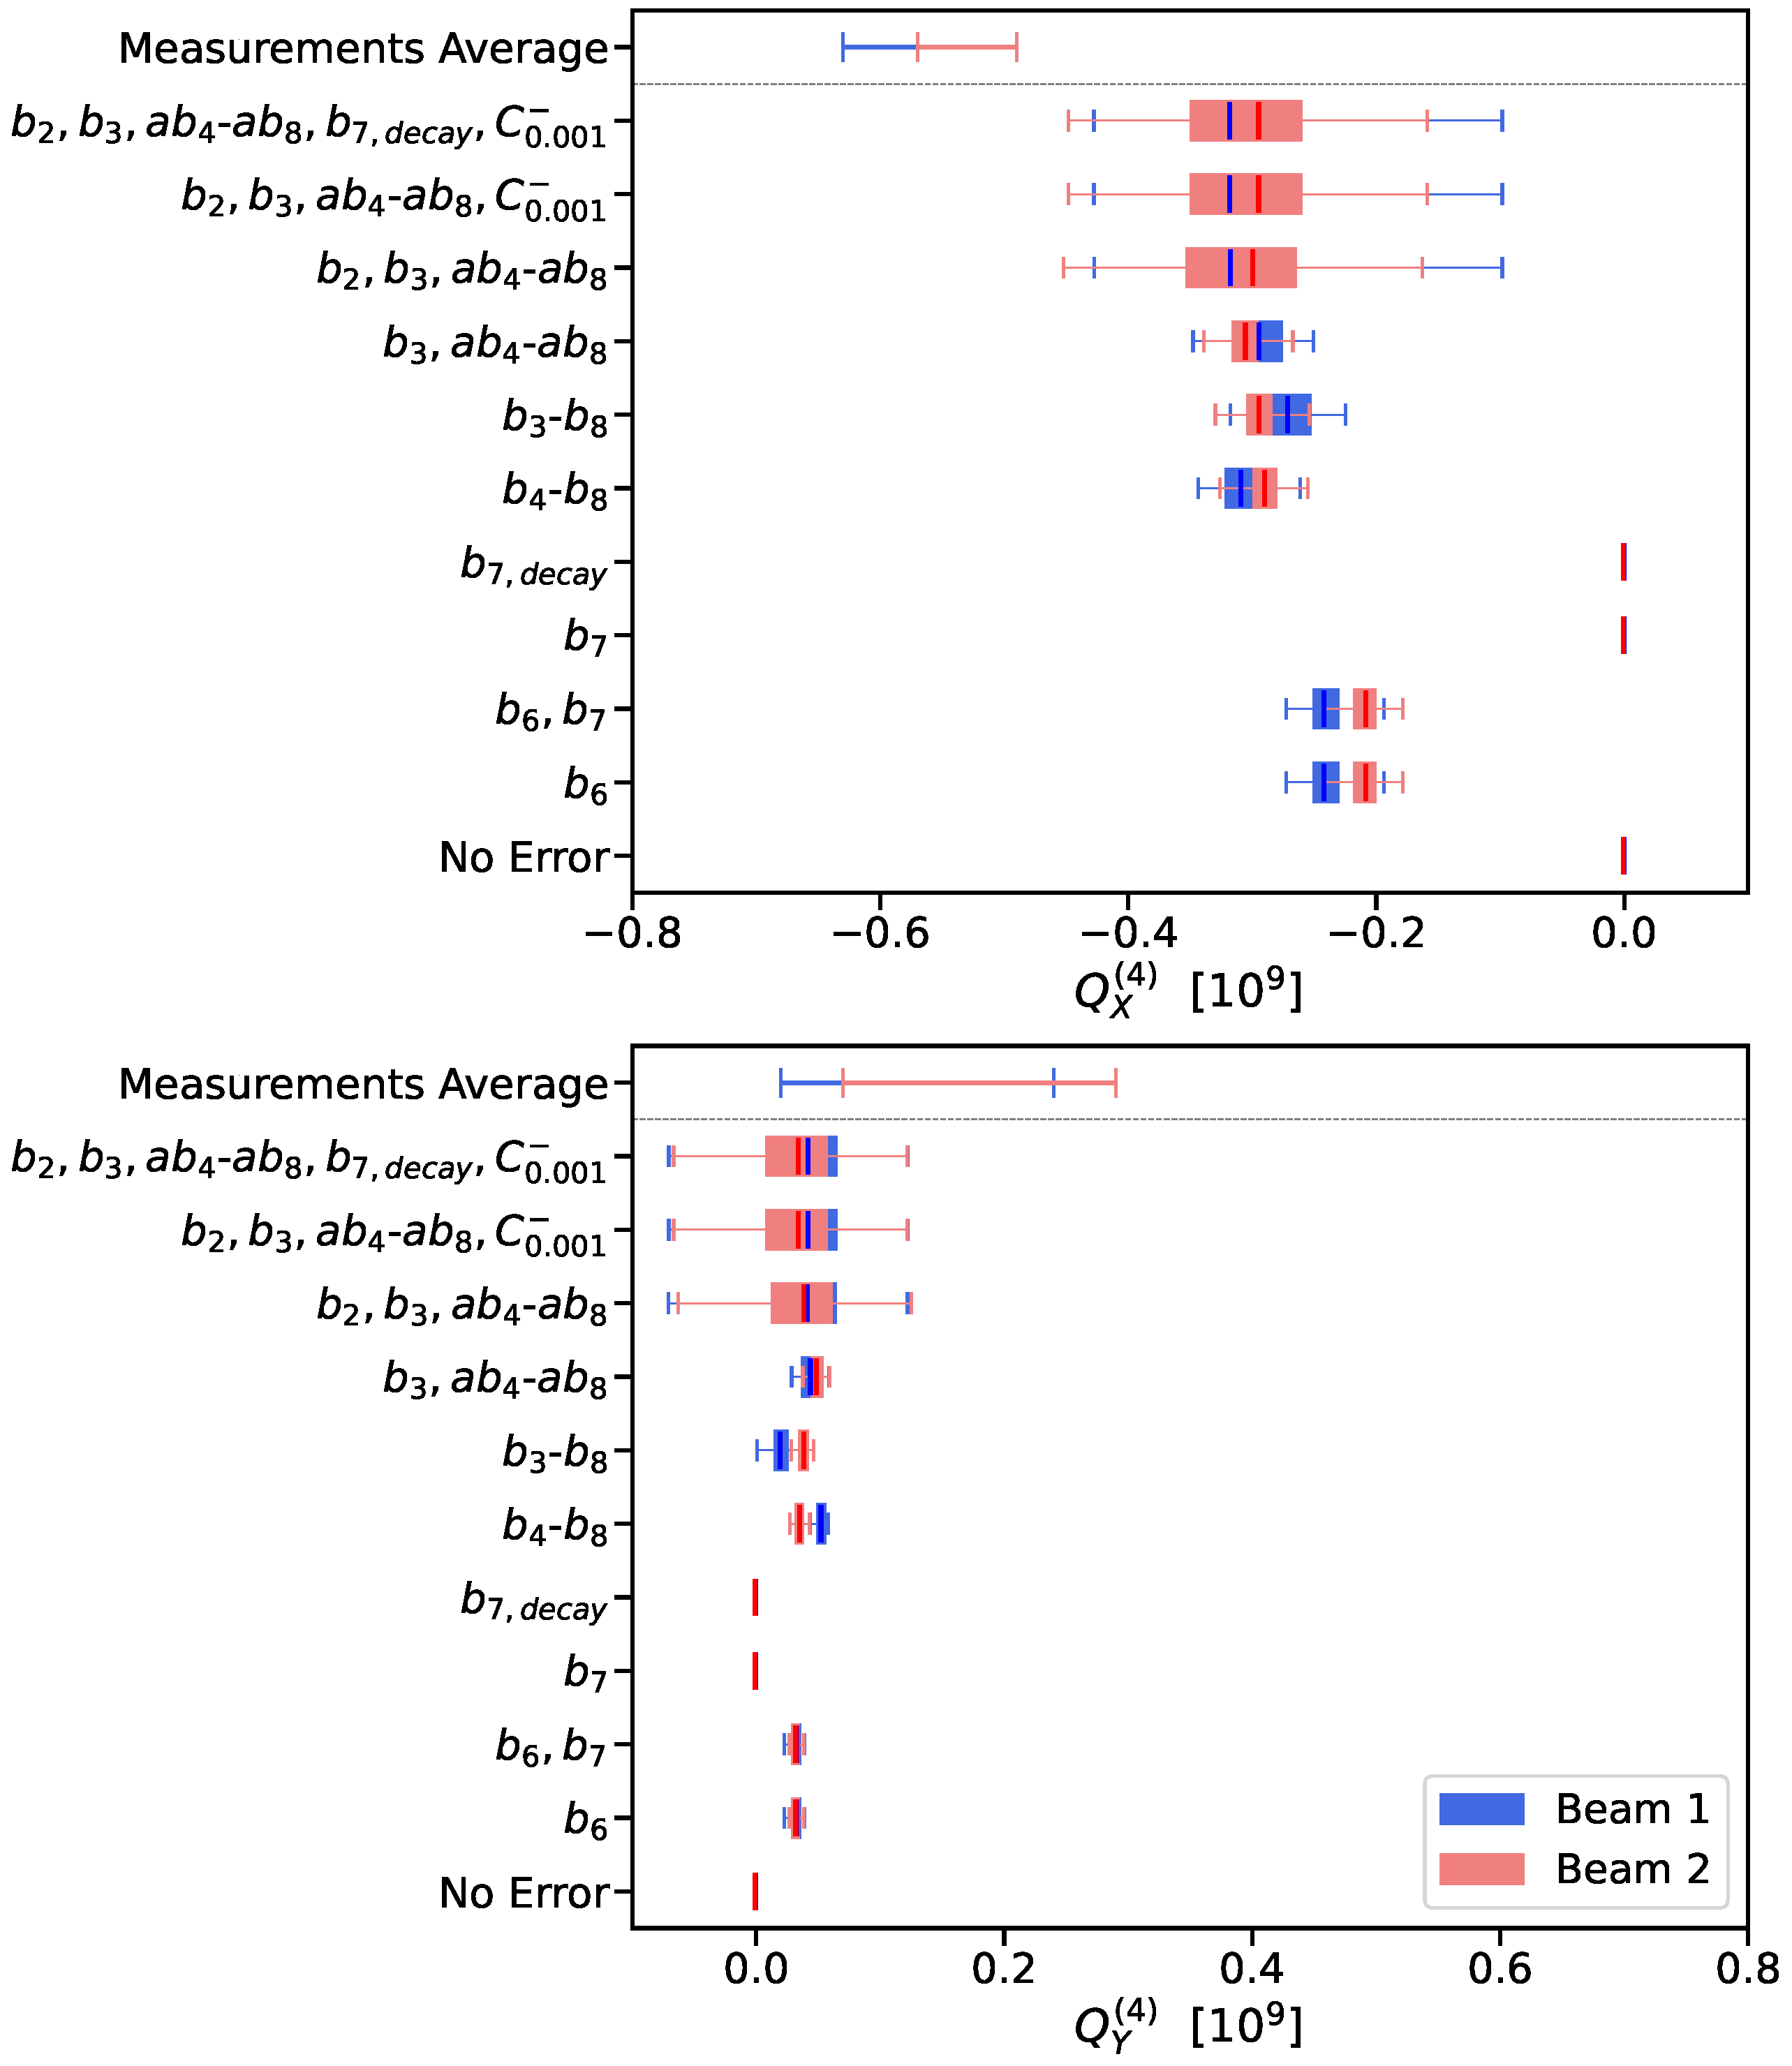
\includegraphics[width=0.9\columnwidth]{images/q4_ptc.pdf}
    \caption{Measured and simulated fourth order chromaticity with different multipole errors. The
    $b_2$ errors, applied on dipoles and quadrupoles, generate beta-beating. Coupling is set to a
    value commonly seen in operation.}
    \label{fig:high_orders:beam1_q4_ptc}
\end{figure}



% ----------------------------------
%\FloatBarrier
\paragraph{\review{Fifth Order Chromaticity}}

It is seen that the the decatetrapolar errors are the main contributors to $Q^{(5)}$, as can be seen
in \cref{fig:high_orders:beam1_q5_ptc}. Fringe fields and skew multipoles have been found to have a
negligible impact. 
Beta-beating and coupling are seen to increase by a small amount the chromaticity, while sextupolar
errors induce a spread with the different seeds. 
Comparing the simulation at the top with most errors added, the $b_7$ component alone accounts for
$\approx 70\%$ of it for both axes on each beam.

\begin{figure}[!htb]
    \centering
    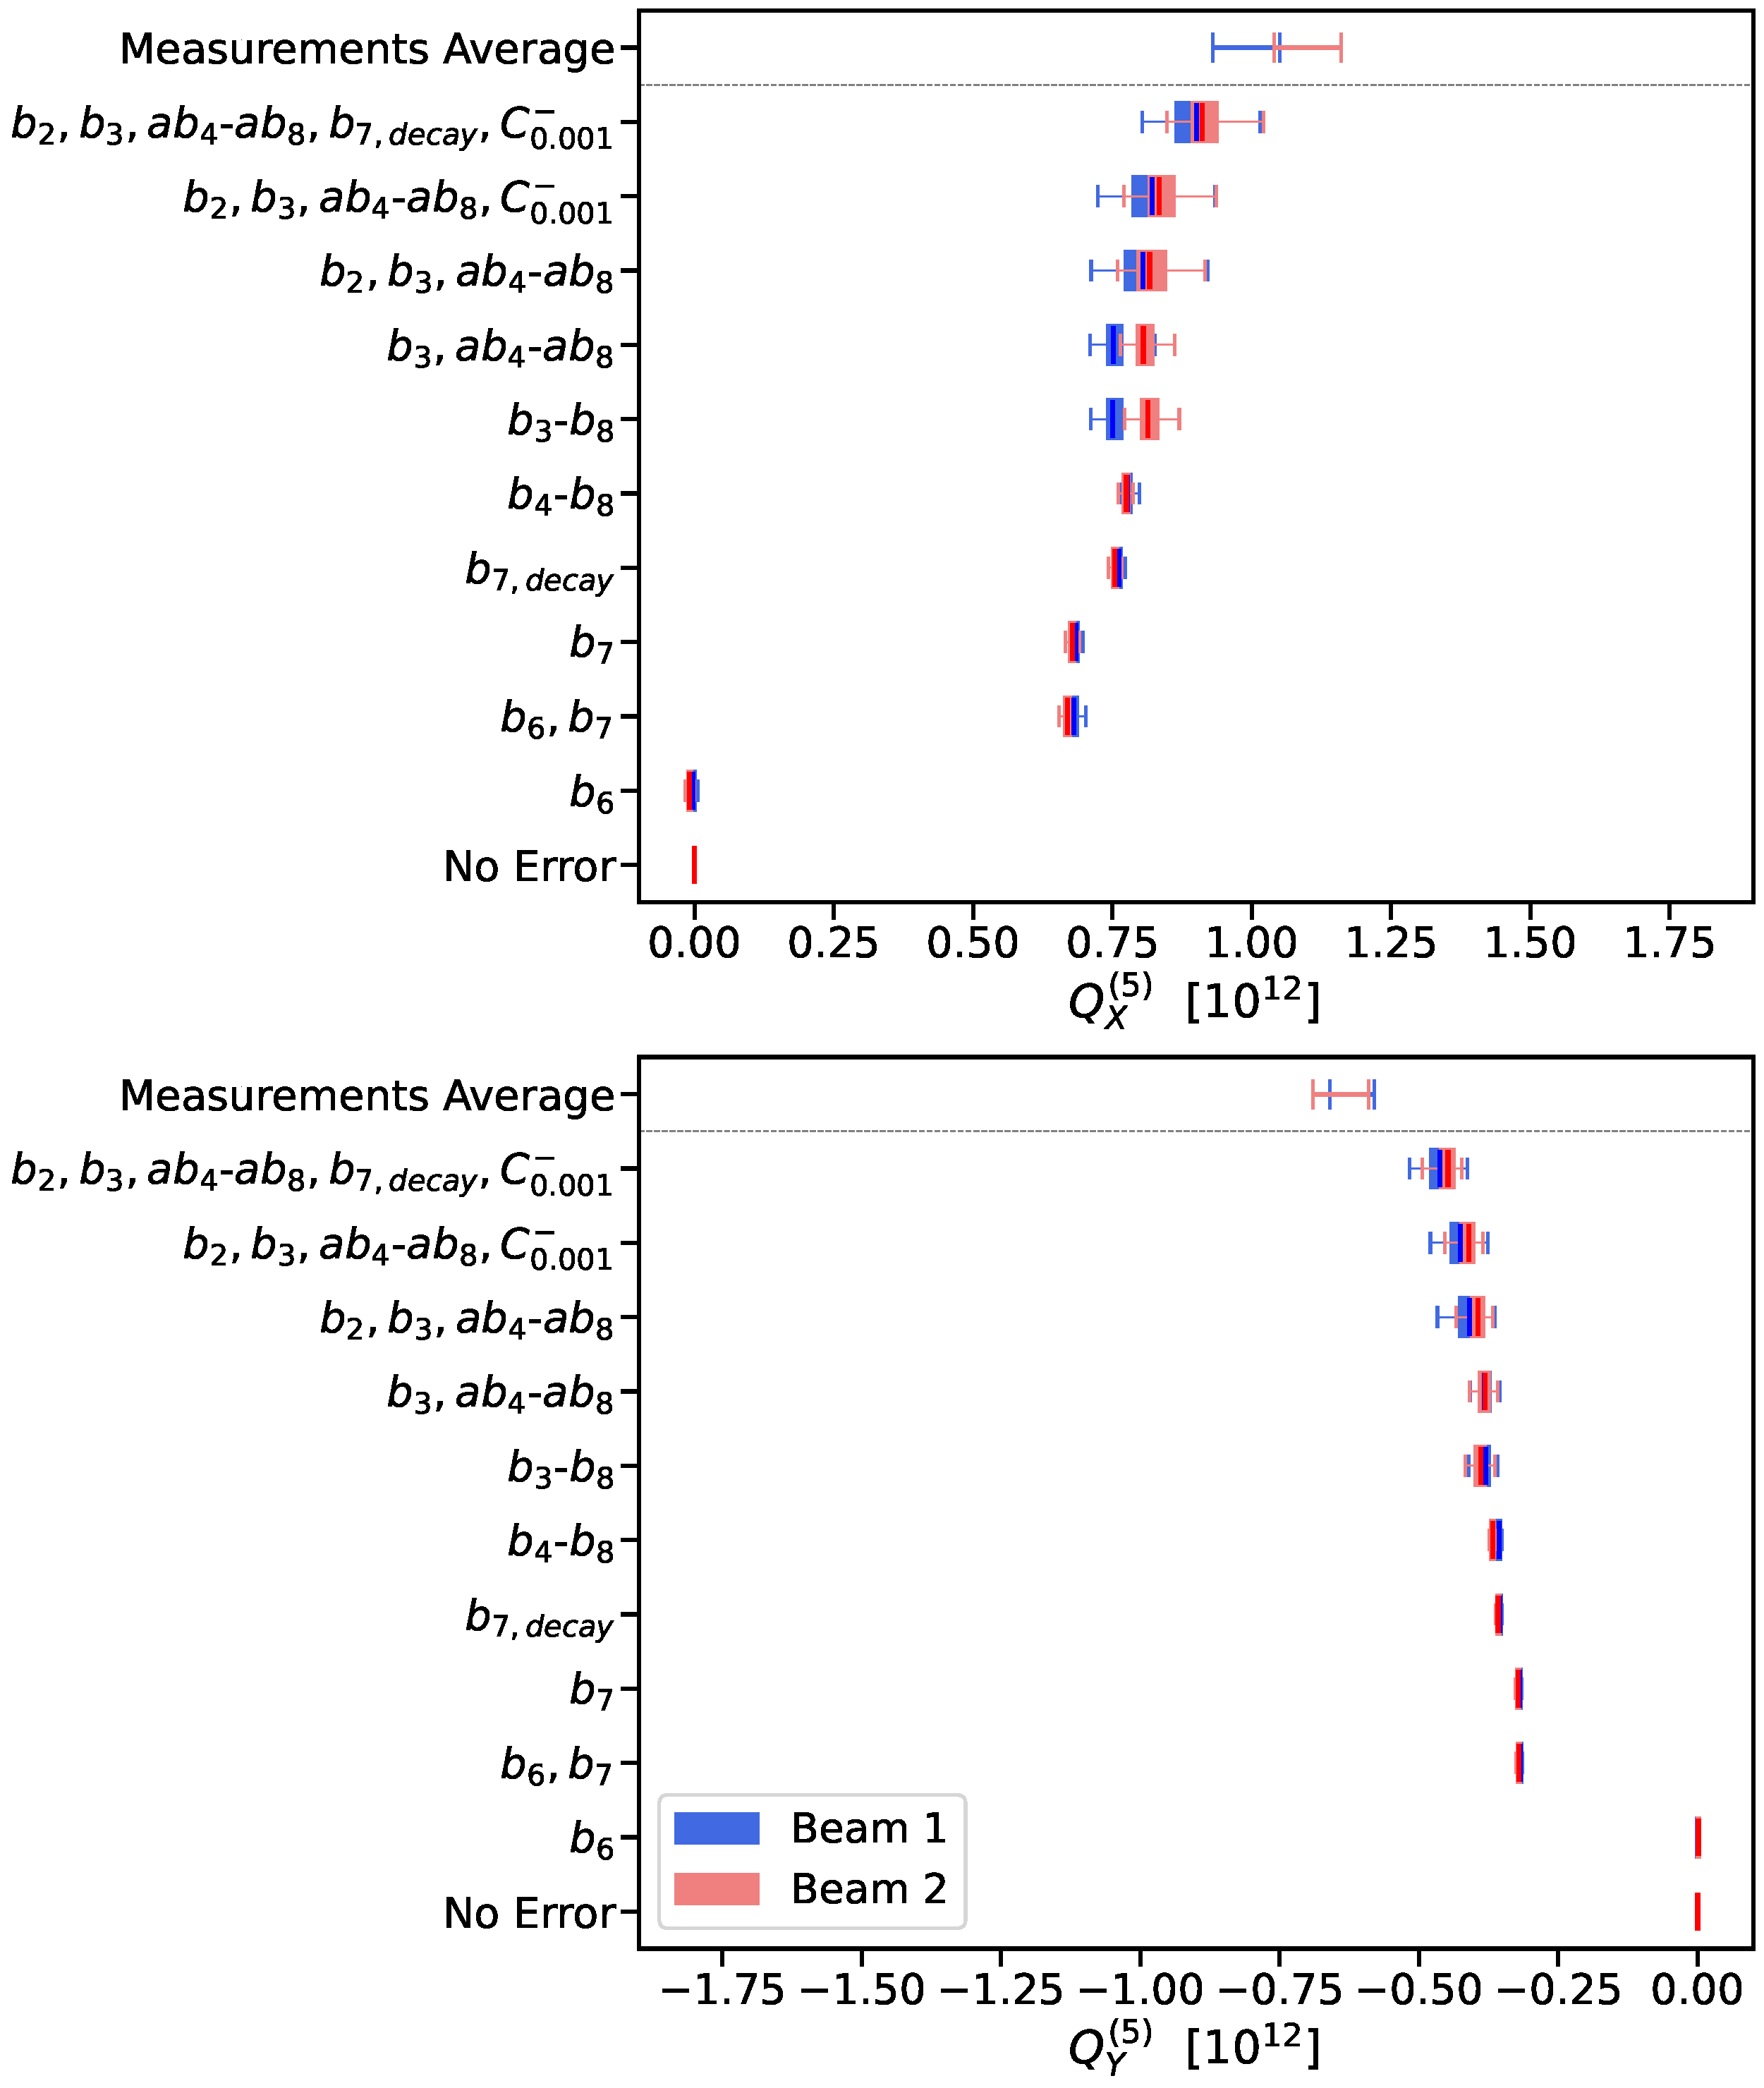
\includegraphics[width=0.9\columnwidth]{images/q5_ptc.pdf}
    \caption{Measured and simulated fifth order chromaticity with different multipole errors. The
    $b_2$ errors, applied on dipoles and quadrupoles, generate beta-beating. Coupling is set to a
    value commonly seen in operation.}
    \label{fig:high_orders:beam1_q5_ptc}
\end{figure}


% Decay
It has been noted in the previous chapter about decapoles (see \cref{section:decapoles:decay}) that
the $b_5$ component in the main dipoles was large at injection energy, and could explain most of the
discrepancy between the measurements and simulations.
Such a decay in the main dipoles also exists for the $b_7$ component~\cite{deniau2024private}, and
is shown in \cref{fig:high_orders:b7_decay}. 

\begin{figure}[!htb]
    \centering
    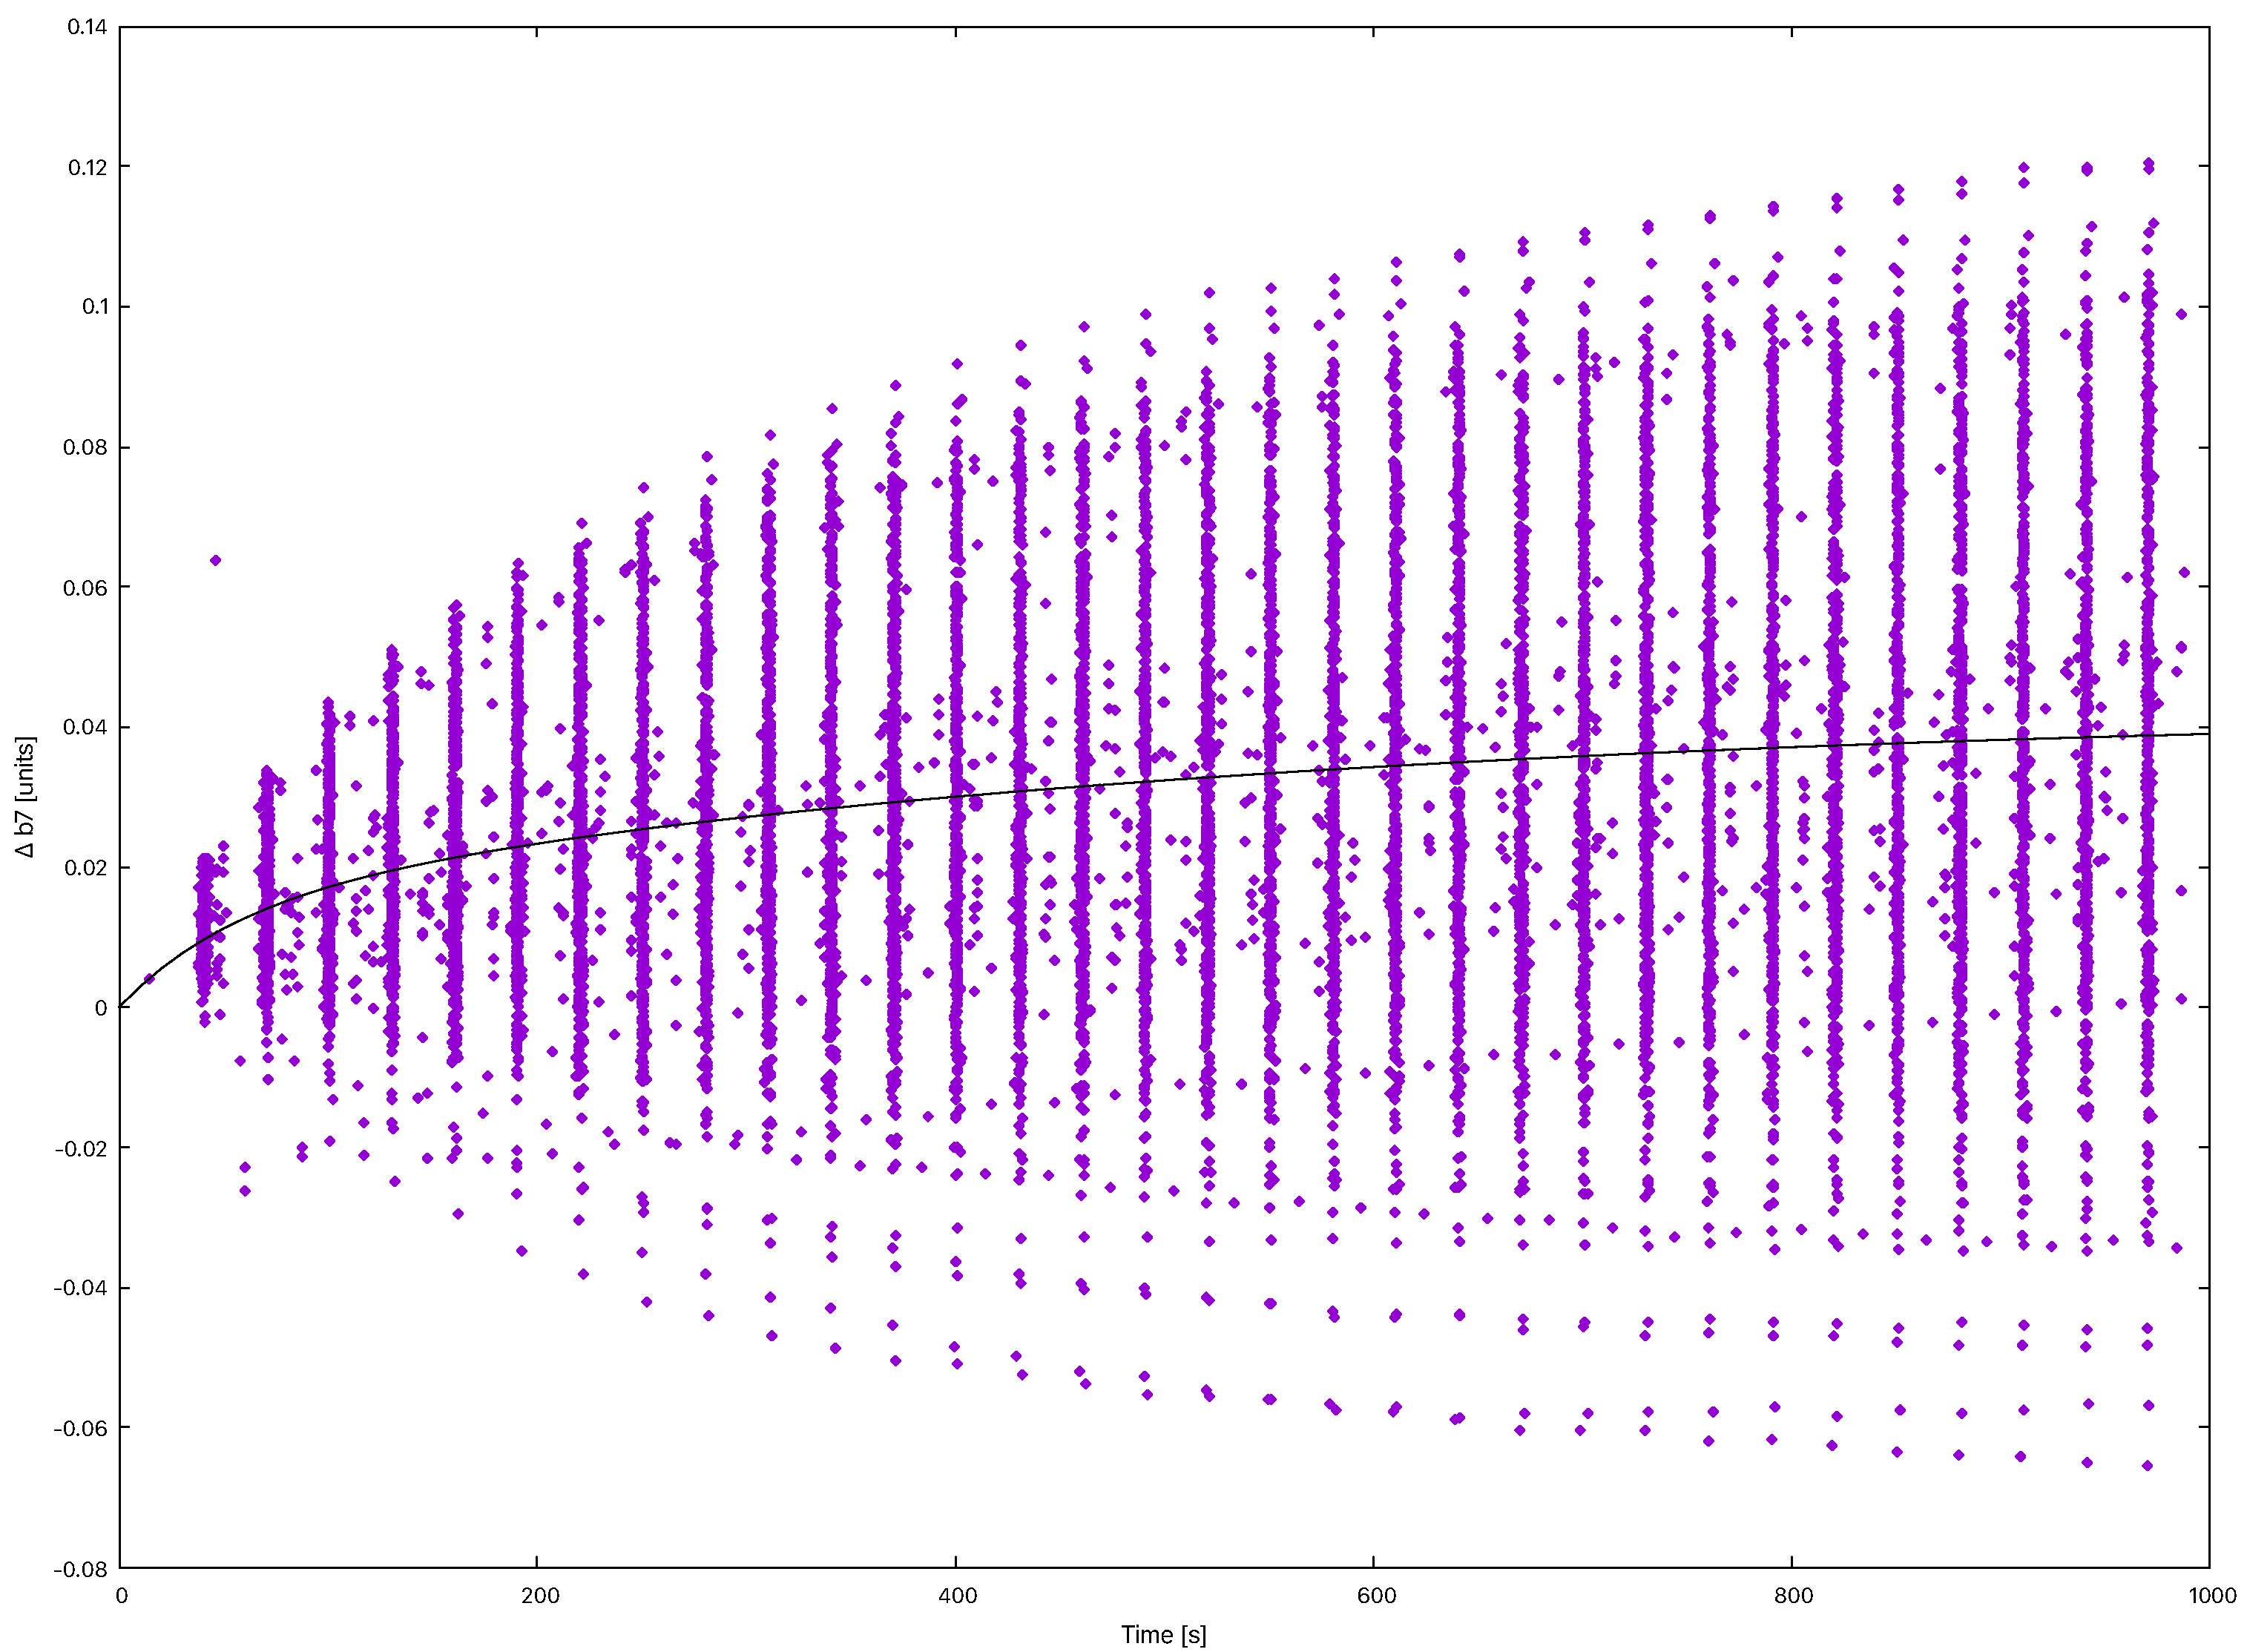
\includegraphics[width=0.9\columnwidth]{images/decay_b7.pdf}
    \caption{Measured decay of the integrated decatetrapolar field in LHC's main dipoles at
    injection energy. The fit is shown in black~\cite{deniau2024private} and settles around
    $+0.035$.}
    \label{fig:high_orders:b7_decay}
\end{figure}

Its value is though small and settles around $+0.0351 \pm 0.0007$. The average $b_7$ of the main
dipoles is of $0.32 \pm 0.16$. The decay thus increase that value of only about $11\%$.
Simulations done with that decay taken into account are also present in the previous
\cref{fig:high_orders:beam1_q5_ptc}.


%----------------------------------------
%       Agreement with Measurements
\FloatBarrier
\subsubsection{\review{Agreement with Measurements}}

Previous simulation results are shown in \cref{tab:high_orders:ptc_values}, taking the values from 
the simulation including the most effects at the top of the plots. For the fourth order, the beating
is not included as the large induced $Q^{(4)}$ is not yet explained.
\Cref{tab:high_orders:ptc_values_ratios} shows the ratio between the measured average and simulated
chromaticities.

\begin{table}[!htb]
  \centering
  \begin{tabular}{lrr}
  \toprule
      Plane     &  $Q^{(4)} [10^9]$  &  $Q^{(5)} [10^{12}]$ \\
  \midrule
      Beam 1    &              &               \\
      \hspace{2mm}X         & $-0.29 \pm 0.02$ & $ 0.90 \pm 0.05$  \\
      \hspace{2mm}Y         & $ 0.04 \pm 0.01$ & $-0.46 \pm 0.03$  \\
      Beam 2    &  &   \\
      \hspace{2mm}X         & $-0.31 \pm 0.02$ & $ 0.92 \pm 0.03$ \\
      \hspace{2mm}Y         & $ 0.05 \pm 0.00$ & $-0.45 \pm 0.01$ \\
  \bottomrule
  \end{tabular}
  \caption{Simulated high order chromaticity terms via PTC at injection energy, including normal and
  skew sextupolar to decahexapolar field errors. Are also included beta-beating, coupling and
  decatetrapolar decay. For the fourth order, the values do not include beta-beating as the observed
  spread is not yet fully understood.}
  \label{tab:high_orders:ptc_values}
\end{table}

%\begin{table}[!htb]
%  \centering
%  \footnotesize
%  \begin{tabular}{lcccc}
%    \toprule
%                    &  \multicolumn{2}{c}{$Q^{(4)}$ Ratio}   &  \multicolumn{2}{c}{$Q^{(5)}$ Ratio} \\
%    \cmidrule(lr){2-3}\cmidrule(lr){4-5}
%      Plane         & First Meas.  & Second Meas.& First Meas.& Second Meas. \\ 
%    \midrule
%      Beam 1        &           &             &            & \\
%      \hspace{2mm}X &  $1.91\pm0.15$ & $2.15\pm0.17$    & $1.33\pm0.10$  & $1.35\pm0.09$   \\
%      \hspace{2mm}Y &  $3.50\pm0.90$ & $0.90\pm0.50$    & $1.91\pm0.22$  & $1.21\pm0.11$   \\
%      Beam 2        &                   &               &     & \\
%      \hspace{2mm}X &                & $4.90\pm1.00$    &                & $1.17\pm0.08$   \\
%      \hspace{2mm}Y &  $1.90\pm0.12$ & $3.30\pm0.50$    & $1.65\pm0.29$  & $1.47\pm0.12$   \\
%      \bottomrule
%  \end{tabular}
%  \caption{Ratios of the simulated and measured high order chromaticity terms for both the first and
%  second performed measurements. The values are taken from tables
%  \cref{tab:high_orders:chroma_fidel}, \cref{tab:high_orders:chroma_table_after} and
%  \cref{tab:high_orders:ptc_values}. The fit with high correlation between both terms is not
%  included.}
%  \label{tab:high_orders:ptc_values_ratios}
%\end{table}

\begin{table}[!htb]
    \centering
    \begin{tabular}{lcc}
      \toprule
        Plane         & $Q^{(4)}$ Ratio&  $Q^{(5)}$ Ratio \\
      \midrule
        Beam 1        &                &                  \\
        % Via weighted mean, which is probably not right.
        %\hspace{2mm}X &  $1.98\pm0.16$ & $1.10\pm0.09$    \\
        %\hspace{2mm}Y &  $3.00\pm0.70$ & $1.34\pm0.11$    \\
        \hspace{2mm}X &  $1.91\pm0.28$ & $1.24\pm0.23$    \\
        \hspace{2mm}Y &  $3.00\pm2.60$ & $1.47\pm0.27$    \\
        Beam 2        &                &                  \\
        %\hspace{2mm}X &  $1.74\pm0.11$ & $1.20\pm0.08$    \\
        %\hspace{2mm}Y &  $2.90\pm0.50$ & $1.42\pm0.12$    \\
        \hspace{2mm}X &  $1.74\pm0.16$ & $1.34\pm0.29$    \\
        \hspace{2mm}Y &  $3.70\pm2.30$ & $1.51\pm0.14$    \\
        \bottomrule
    \end{tabular}
    \caption{Ratios of the simulated and average measured high-order chromaticity terms.  The values
    are taken from \cref{fig:high_oders:all_values} and \cref{tab:high_orders:ptc_values}.}
    \label{tab:high_orders:ptc_values_ratios}
\end{table}

The similar ratios between planes and beams for the fifth order could indicate a systematic error
not modeled.
The large differences observed for the fourth order are not yet explained but the difference between
planes could be linked to a shift induced by the decapolar corrections in the vertical plane. It
indeed seems that the fourth order follows a trend with the third order.
%\todo{check correlation between Q3 Q4}



%=============================
%       Model Estimates
%=============================
\section{\review{Model Estimates}}
\label{sec:nl_chroma_model}


The model of the LHC is based on MAD-X and WISE field errors~\cite{p_hagen_wise_2006}, containing
a hundred seeds for the random errors. To compute the chromaticity, simulations are run via PTC,
with various field errors.


%====================
\subsection{\review{Decatetrapolar Decay}}

It has been noted in the previous chapter about decapoles (see \cref{section:decapoles:decay}) that
the $b_5$ component in the main dipoles was large at injection energy, and could explain most of the
discrepancy between the measurements and simulations.
Such a decay in the main dipoles also exists for the $b_7$ component~\cite{deniau2024private}, and
is shown in \cref{fig:high_orders:b7_decay}. 

\begin{figure}[!htb]
    \centering
    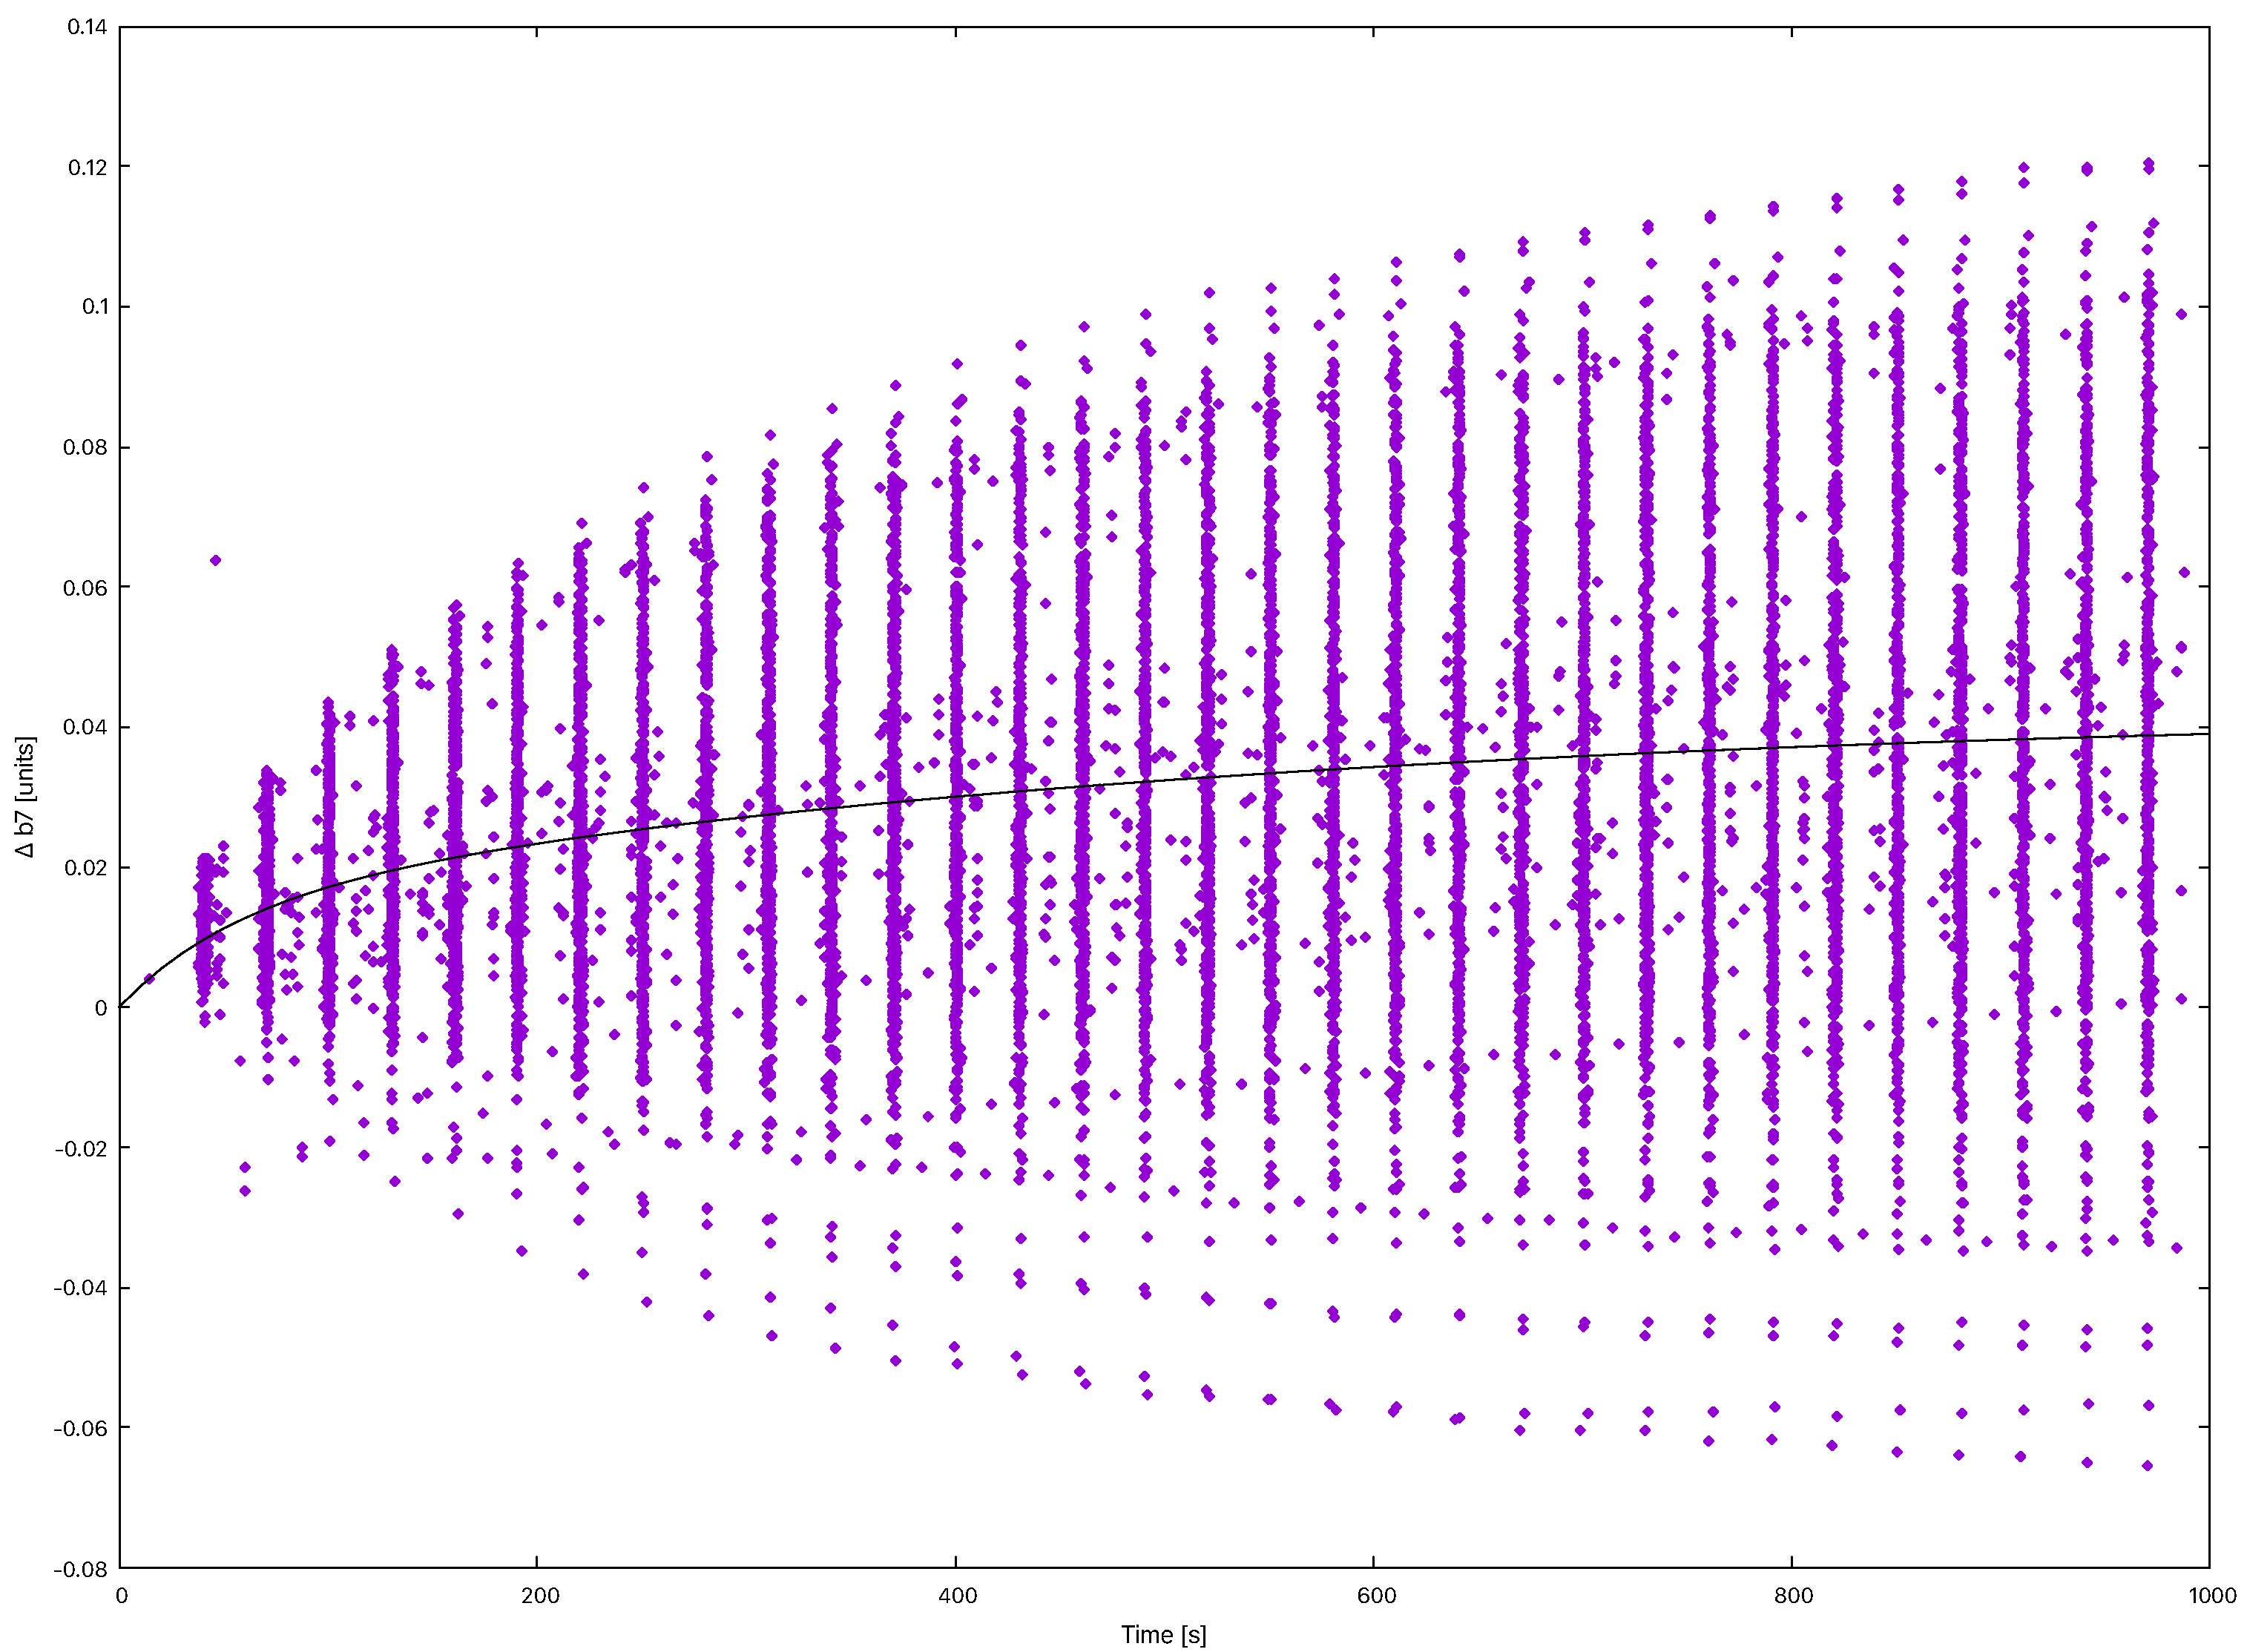
\includegraphics[width=0.9\columnwidth]{images/decay_b7.pdf}
    \caption{Measured decay of the integrated decatetrapolar field in LHC's main dipoles at
    injection energy. The fit is shown in black~\cite{deniau2024private} and settles around
    $+0.035$.}
    \label{fig:high_orders:b7_decay}
\end{figure}

Its value is though small and settles around $+0.0351 \pm 0.0007$. The average $b_7$ of the main
dipoles is of $0.32 \pm 0.16$. The decay thus increase that value of only about $11\%$.
Simulations done with that decay taken into account are detailed next.


% =================================
\subsection{\review{Major contributions}}

Simulations with various field errors have been run to assess the contribution of individual magnet
order and combinations for the fourth and firth order chromaticity. Normal and skew fields errors
ranging from sextupolar ($b_3$) to decahexapolar ($b_8$) are added alone or in combination to
observe which is the strongest. Quadrupolar field errors ($b_2$) introduce beta-beating. Coupling is
introduced via skew quadrupolar correctors.


% ----------------------------------
\subsubsection{\review{Fourth Order Chromaticity}}

The results from simulations strongly imply that the dodecapolar errors are the main contributors
to $Q^{(4)}$, as can be seen in \cref{fig:high_orders:beam1_q4_ptc}.
Fringe fields have a negligible impact, as do skew multipoles.
The most notable effect on this chromaticity order is the beta-beating, introducing a very large
spread via the various error seeds.
Comparing the simulation at the top with most errors added, the $b_6$ component alone accounts for
$\approx 70\%$ of it for both axes on each beam.

\begin{figure}[!htb]
    \centering
    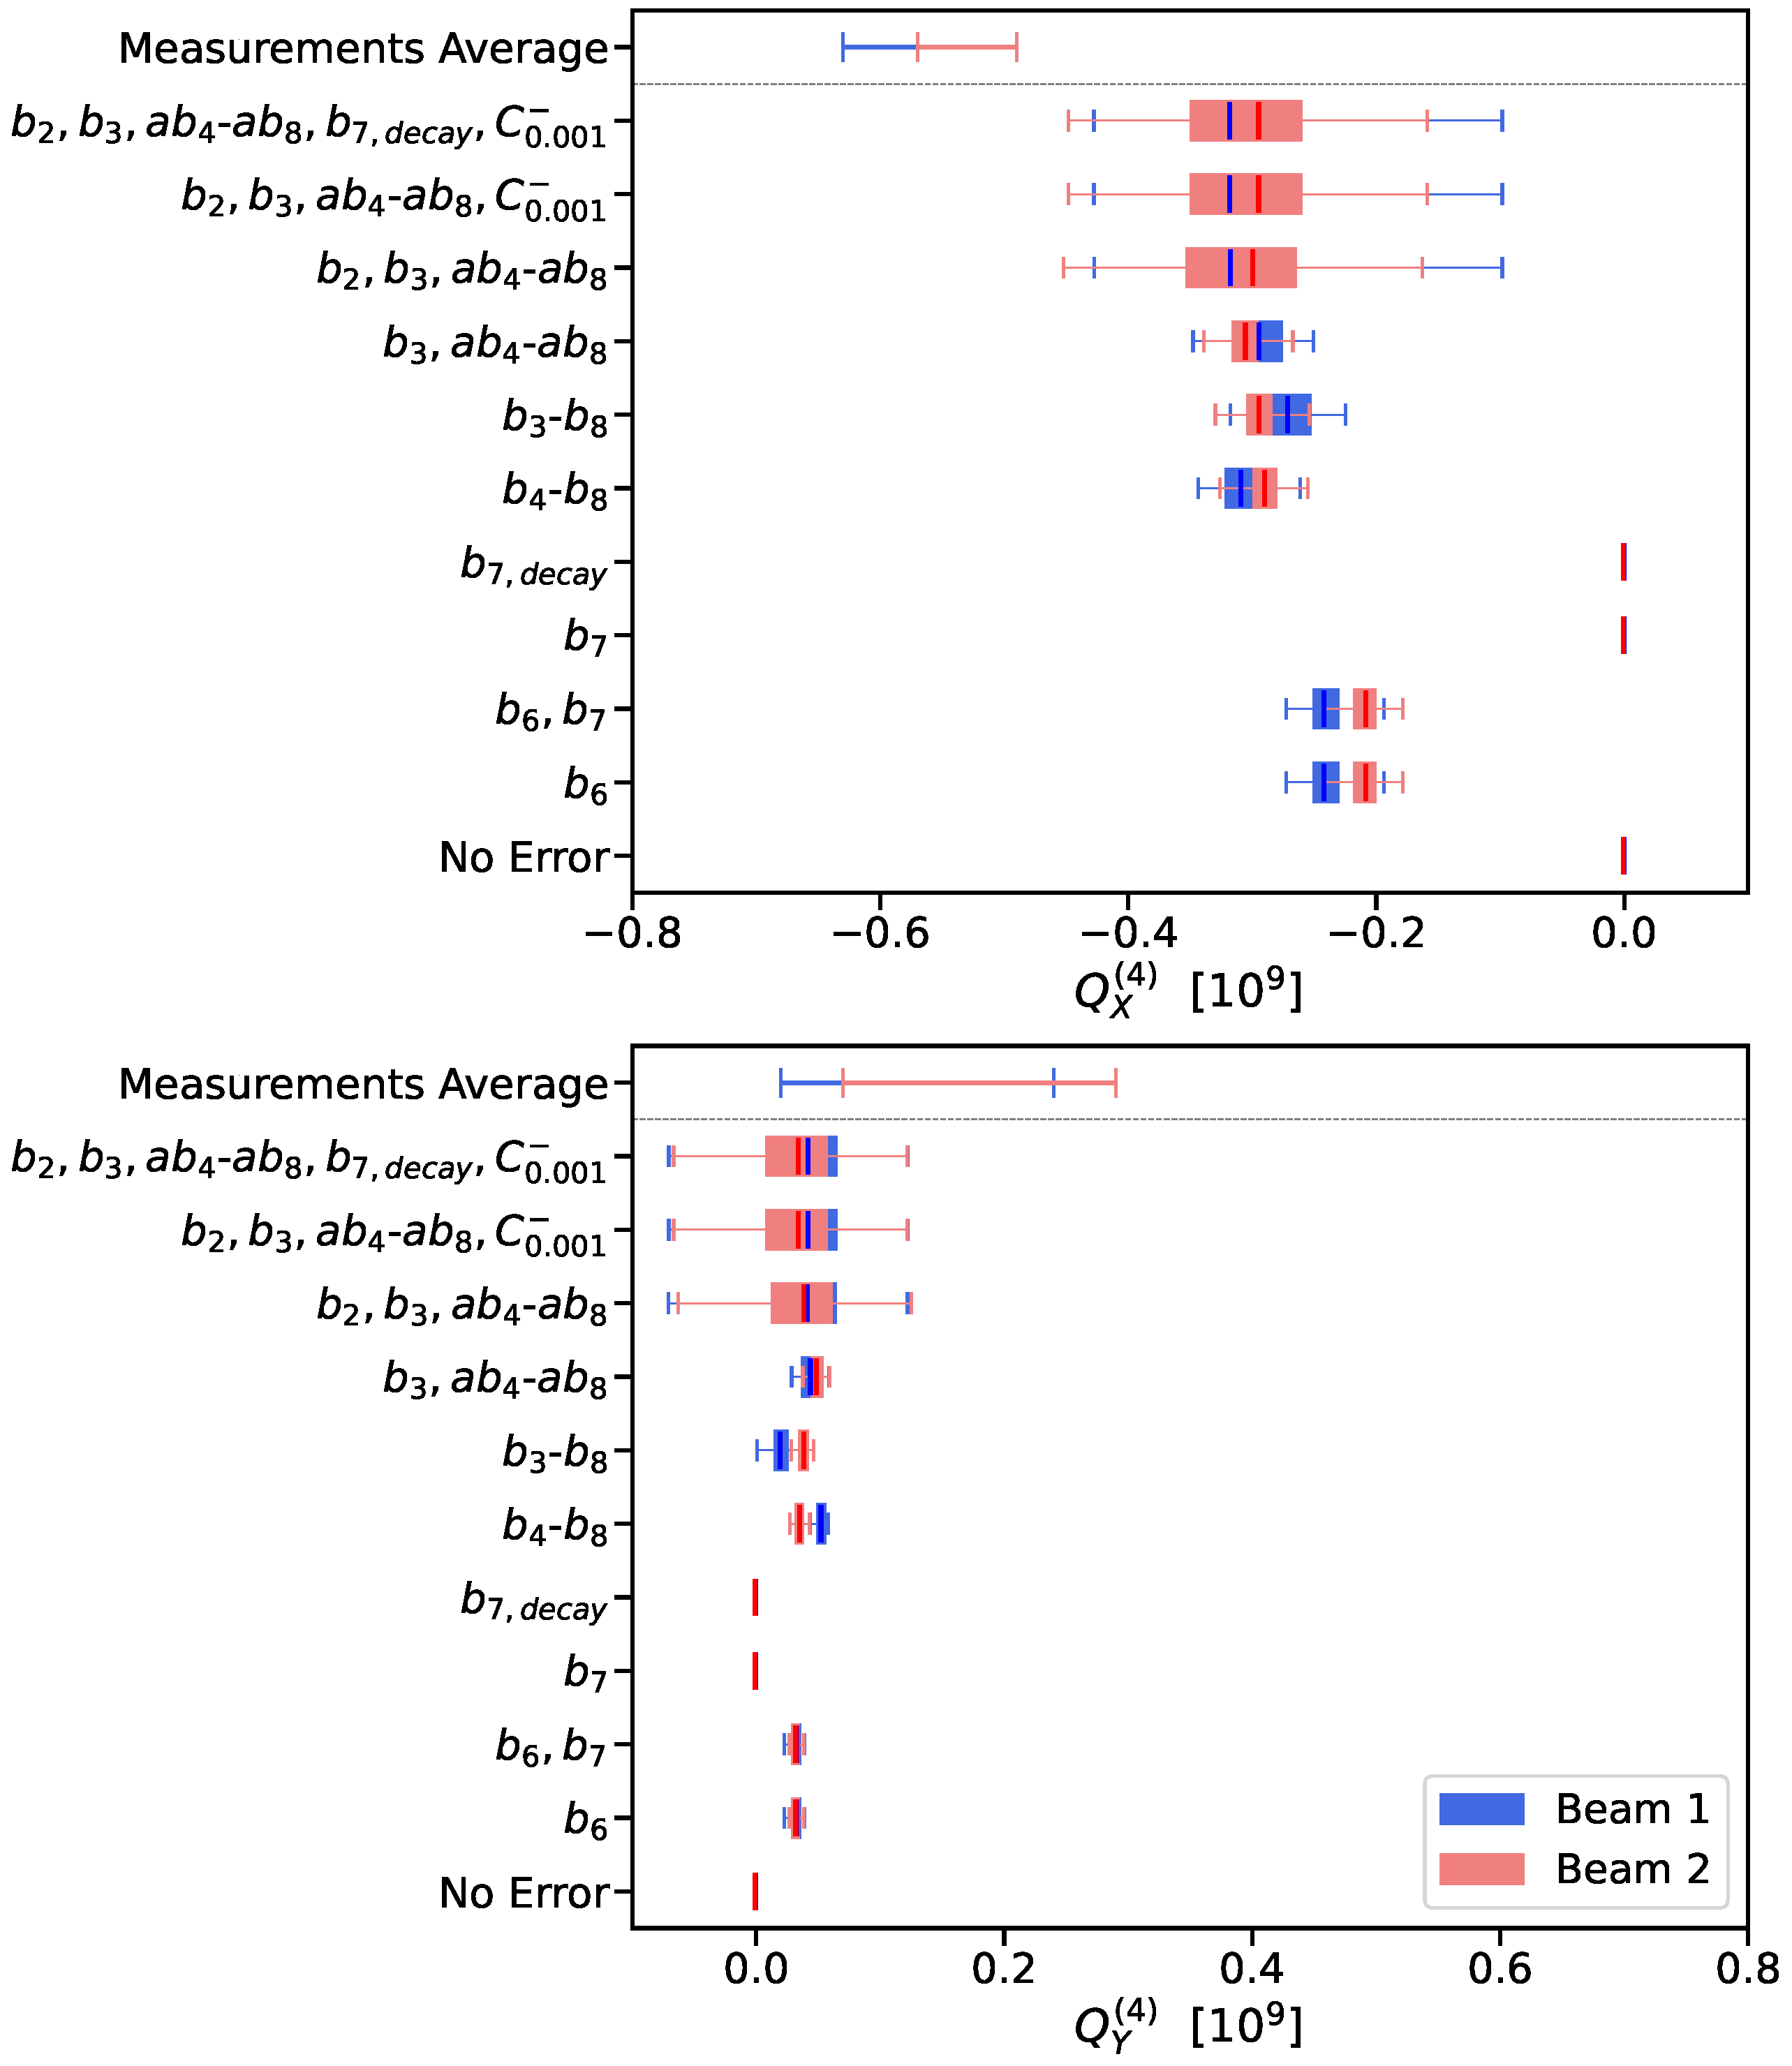
\includegraphics[width=0.9\columnwidth]{images/q4_ptc.pdf}
    \caption{Measured and simulated fourth order chromaticity with different multipole errors. The
    $b_2$ errors, applied on dipoles and quadrupoles, generate beta-beating. Coupling is set to a
    value commonly seen in operation.}
    \label{fig:high_orders:beam1_q4_ptc}
\end{figure}



% ----------------------------------
\subsubsection{\review{Fifth Order Chromaticity}}

It is seen that the the decatetrapolar errors are the main contributors to $Q^{(5)}$, as can be seen
in \cref{fig:high_orders:beam1_q5_ptc}. Fringe fields and skew multipoles have been found to have a
negligible impact. 
Beta-beating and coupling are seen to increase by a small amount the chromaticity, while sextupolar
errors induce a spread with the different seeds. 
As for the fourth order, comparing the simulation at the top with most errors added, the $b_7$
component alone accounts for $\approx 70\%$ of it for both axes on each beam of the fifth order
chromaticity.

\begin{figure}[!htb]
    \centering
    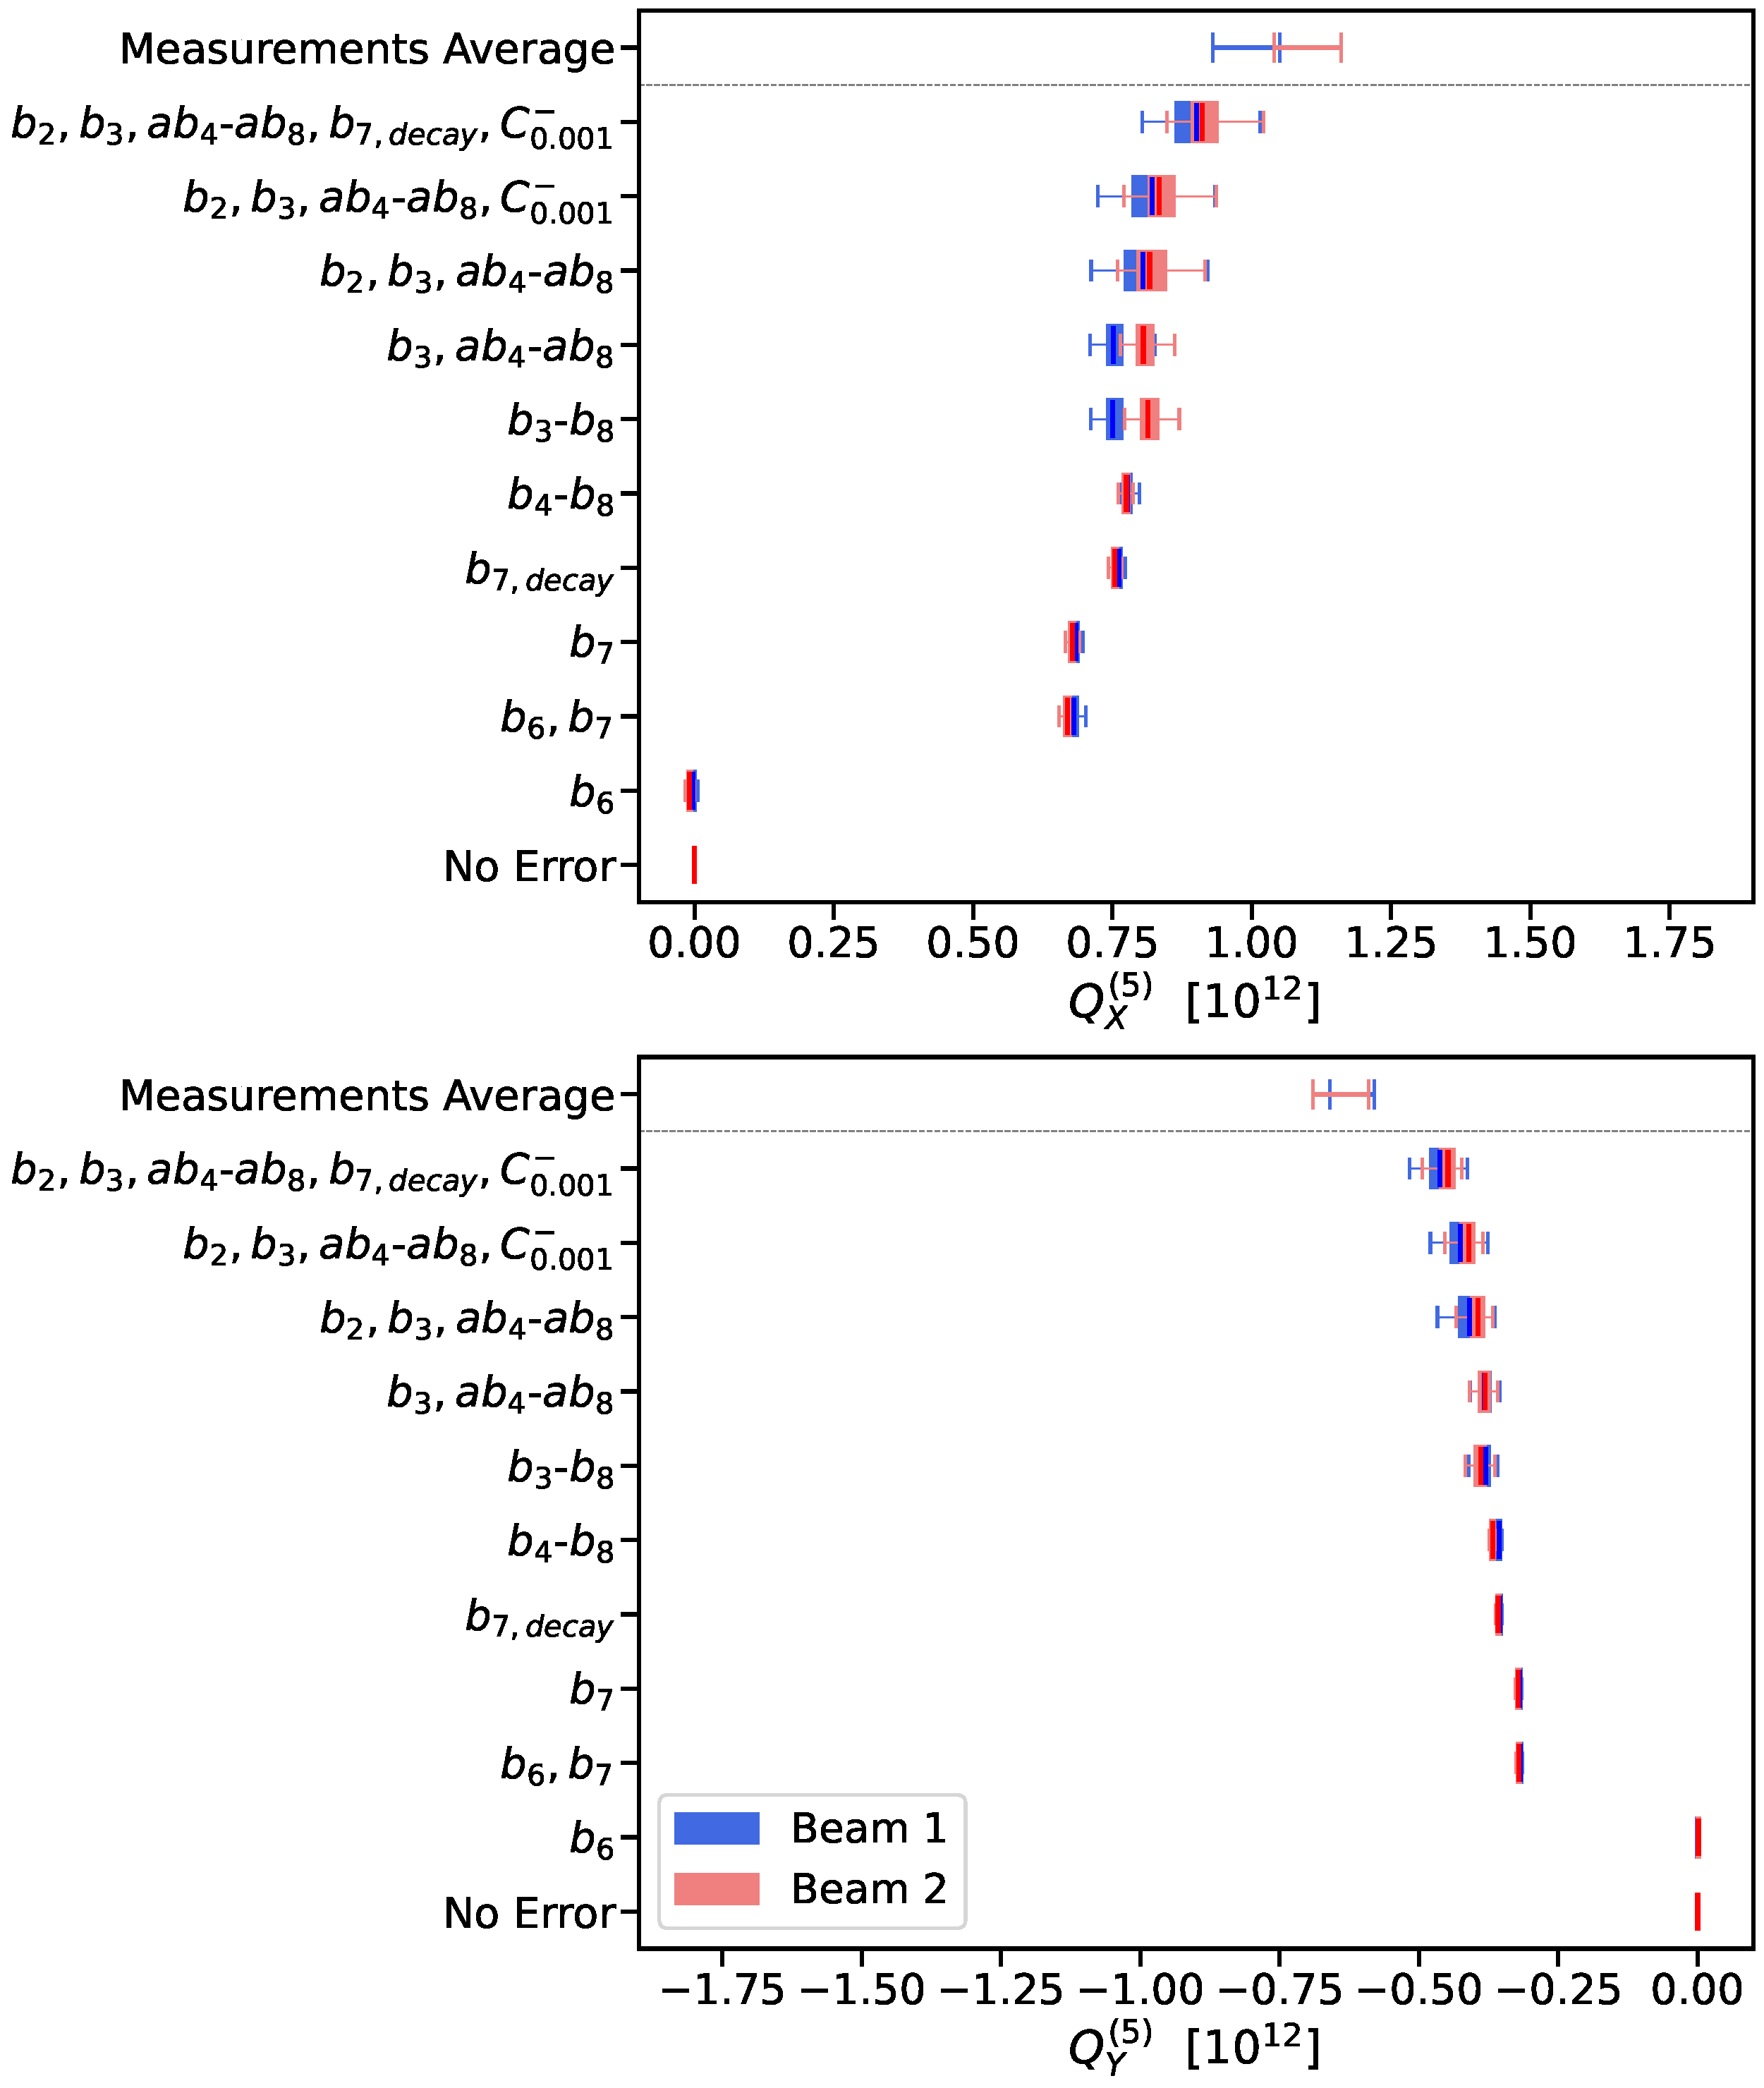
\includegraphics[width=0.9\columnwidth]{images/q5_ptc.pdf}
    \caption{Measured and simulated fifth order chromaticity with different multipole errors. The
    $b_2$ errors, applied on dipoles and quadrupoles, generate beta-beating. Coupling is set to a
    value commonly seen in operation.}
    \label{fig:high_orders:beam1_q5_ptc}
\end{figure}



% =================================
\subsection{\review{Ratios}}

Previous simulation results are shown in \cref{tab:high_orders:ptc_values}, taking the values from 
the simulation including the most effects at the top of the plots. For the fourth order, the beating
is not included as the large beating is not yet explained.
\Cref{tab:high_orders:ptc_values_ratios} shows the ratio between the measured average and simulated
chromaticities.

\begin{table}[!htb]
  \centering
  \begin{tabular}{lrr}
  \toprule
      Plane     &  $Q^{(4)} [10^9]$  &  $Q^{(5)} [10^{12}]$ \\
  \midrule
      Beam 1    &              &               \\
      \hspace{2mm}X         & $-0.29 \pm 0.02$ & $ 0.90 \pm 0.05$  \\
      \hspace{2mm}Y         & $ 0.04 \pm 0.01$ & $-0.46 \pm 0.03$  \\
      Beam 2    &  &   \\
      \hspace{2mm}X         & $-0.31 \pm 0.02$ & $ 0.92 \pm 0.03$ \\
      \hspace{2mm}Y         & $ 0.05 \pm 0.00$ & $-0.45 \pm 0.01$ \\
  \bottomrule
  \end{tabular}
  \caption{Simulated high order chromaticity terms via PTC at injection energy, including normal and
  skew sextupolar to decahexapolar field errors. Are also included beta-beating, coupling and
  decatetrapolar decay. For the fourth order, the values do not include beta-beating as the observed
  spread is not yet fully understood.}
  \label{tab:high_orders:ptc_values}
\end{table}

%\begin{table}[!htb]
%  \centering
%  \footnotesize
%  \begin{tabular}{lcccc}
%    \toprule
%                    &  \multicolumn{2}{c}{$Q^{(4)}$ Ratio}   &  \multicolumn{2}{c}{$Q^{(5)}$ Ratio} \\
%    \cmidrule(lr){2-3}\cmidrule(lr){4-5}
%      Plane         & First Meas.  & Second Meas.& First Meas.& Second Meas. \\ 
%    \midrule
%      Beam 1        &           &             &            & \\
%      \hspace{2mm}X &  $1.91\pm0.15$ & $2.15\pm0.17$    & $1.33\pm0.10$  & $1.35\pm0.09$   \\
%      \hspace{2mm}Y &  $3.50\pm0.90$ & $0.90\pm0.50$    & $1.91\pm0.22$  & $1.21\pm0.11$   \\
%      Beam 2        &                   &               &     & \\
%      \hspace{2mm}X &                & $4.90\pm1.00$    &                & $1.17\pm0.08$   \\
%      \hspace{2mm}Y &  $1.90\pm0.12$ & $3.30\pm0.50$    & $1.65\pm0.29$  & $1.47\pm0.12$   \\
%      \bottomrule
%  \end{tabular}
%  \caption{Ratios of the simulated and measured high order chromaticity terms for both the first and
%  second performed measurements. The values are taken from tables
%  \cref{tab:high_orders:chroma_fidel}, \cref{tab:high_orders:chroma_table_after} and
%  \cref{tab:high_orders:ptc_values}. The fit with high correlation between both terms is not
%  included.}
%  \label{tab:high_orders:ptc_values_ratios}
%\end{table}

\begin{table}[!htb]
    \centering
    \begin{tabular}{lcc}
      \toprule
        Plane         & $Q^{(4)}$ Ratio&  $Q^{(5)}$ Ratio \\
      \midrule
        Beam 1        &                &                  \\
        % Via weighted mean, which is probably not right.
        %\hspace{2mm}X &  $1.98\pm0.16$ & $1.10\pm0.09$    \\
        %\hspace{2mm}Y &  $3.00\pm0.70$ & $1.34\pm0.11$    \\
        \hspace{2mm}X &  $1.91\pm0.28$ & $1.24\pm0.23$    \\
        \hspace{2mm}Y &  $3.00\pm2.60$ & $1.47\pm0.27$    \\
        Beam 2        &                &                  \\
        %\hspace{2mm}X &  $1.74\pm0.11$ & $1.20\pm0.08$    \\
        %\hspace{2mm}Y &  $2.90\pm0.50$ & $1.42\pm0.12$    \\
        \hspace{2mm}X &  $1.74\pm0.16$ & $1.34\pm0.29$    \\
        \hspace{2mm}Y &  $3.70\pm2.30$ & $1.51\pm0.14$    \\
        \bottomrule
    \end{tabular}
    \caption{Ratios of the simulated and average measured high-order chromaticity terms.  The values
    are taken from \cref{fig:high_oders:all_values} and \cref{tab:high_orders:ptc_values}.}
    \label{tab:high_orders:ptc_values_ratios}
\end{table}

The similar ratios between planes and beams for the fifth order could indicate a systematic error
not modeled.
The large differences observed for the fourth order are not yet explained but the difference between
planes could be linked to a shift induced by the decapolar corrections in the vertical plane. It
indeed seems that the fourth order follows a trend with the third order.
\todo{check correlation between Q3 Q4}


%=============================
%            RDTs
%=============================
\section{\todo{Dodecapolar RDTs}}

\begin{figure}[!htb]
    \centering
    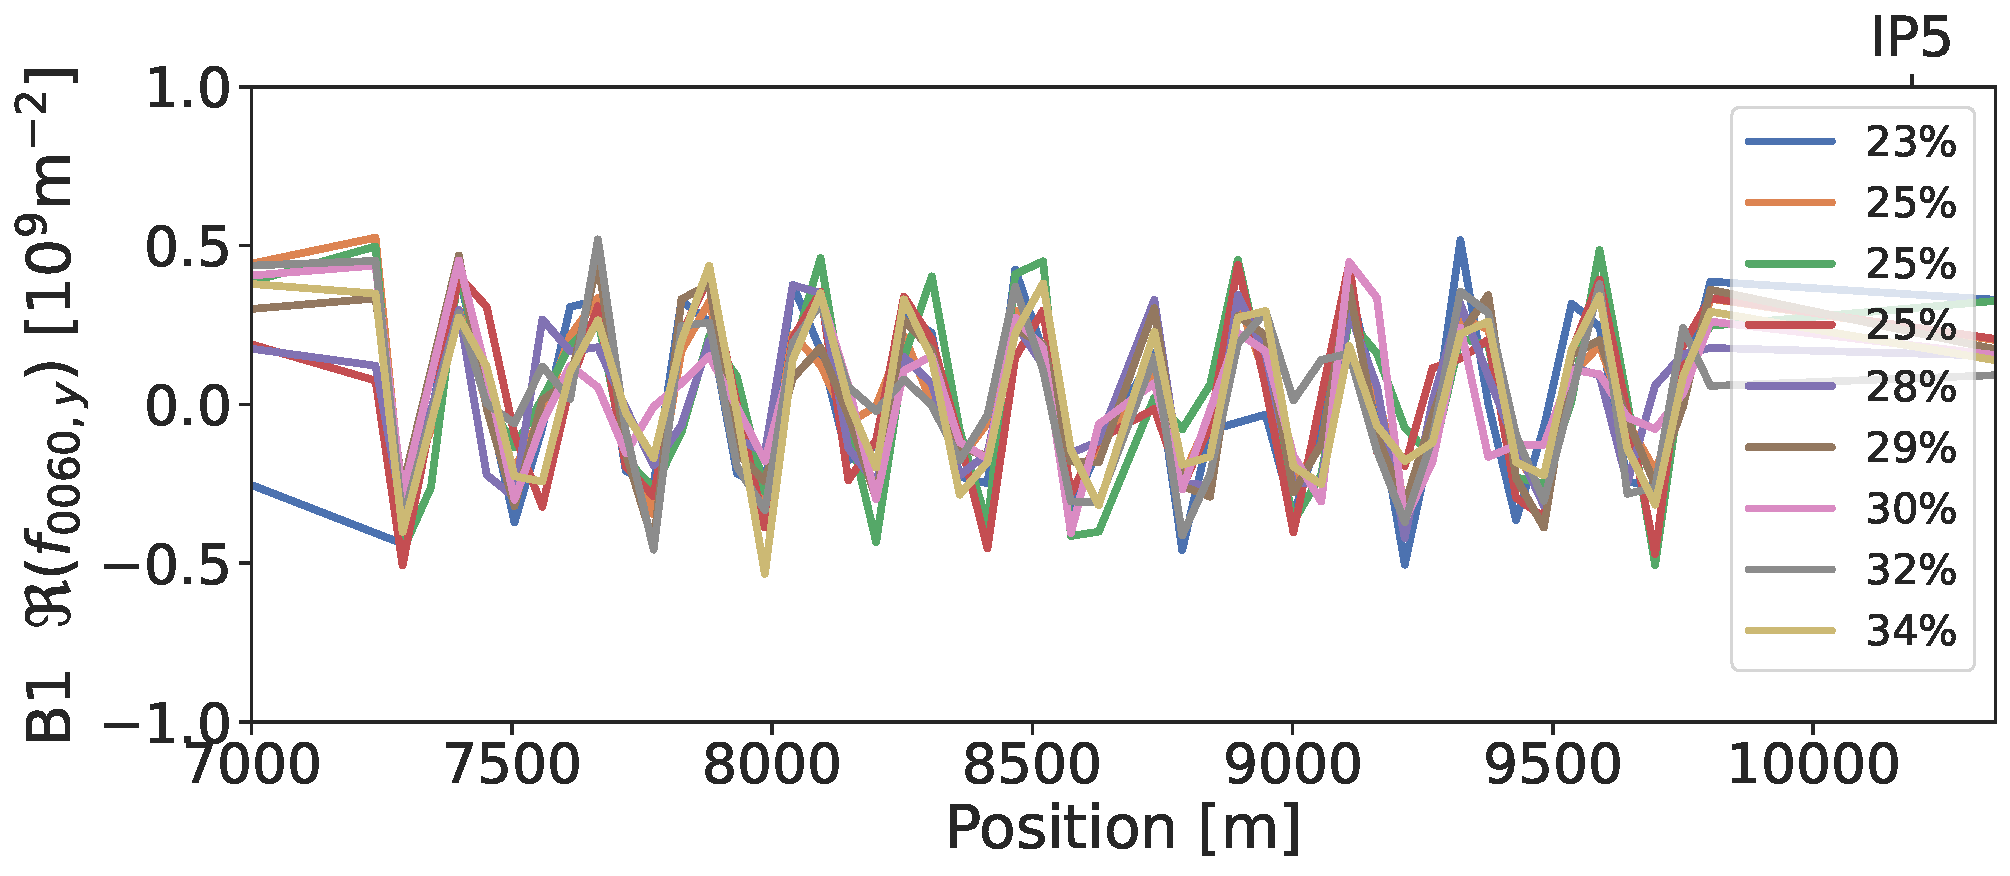
\includegraphics[width=\textwidth]{./images/f0060y_all_meas_real.pdf}
    \caption{Real part of the dodecapolar RDT $f_{0060}$ measured with several kick strengths. The
    RMS amplitude is of $0.35\cdot10^{9}$.}
    \label{fig:high_orders:chroma_nominal_correction_full_range}
\end{figure}





%=============================
%          Further
%=============================
\section{\todo{Going Further}}

% --------------------------------
%          Chromaticity
% --------------------------------
\subsection{\review{Chromaticity}}

% --------------------------------
%          High Ranges
\subsubsection{\review{Limitations}}

So far, the momentum offset ranges of the 2024 measurements have been restricted in order to allow a 
comparison with the shorter ranges measurements made in 2022. The non-linearity of the chromaticity 
and its higher orders become very noticeable once these large ranges are reached.
\Cref{fig:high_orders:chroma_nominal_correction_full_range} shows an example of such measurement for 
Beam 2, made with the nominal corrections, highlighting the difference between two momentum offset
ranges.

\begin{figure}[!htb]
    \begin{subfigure}{0.49\textwidth}
        \centering
        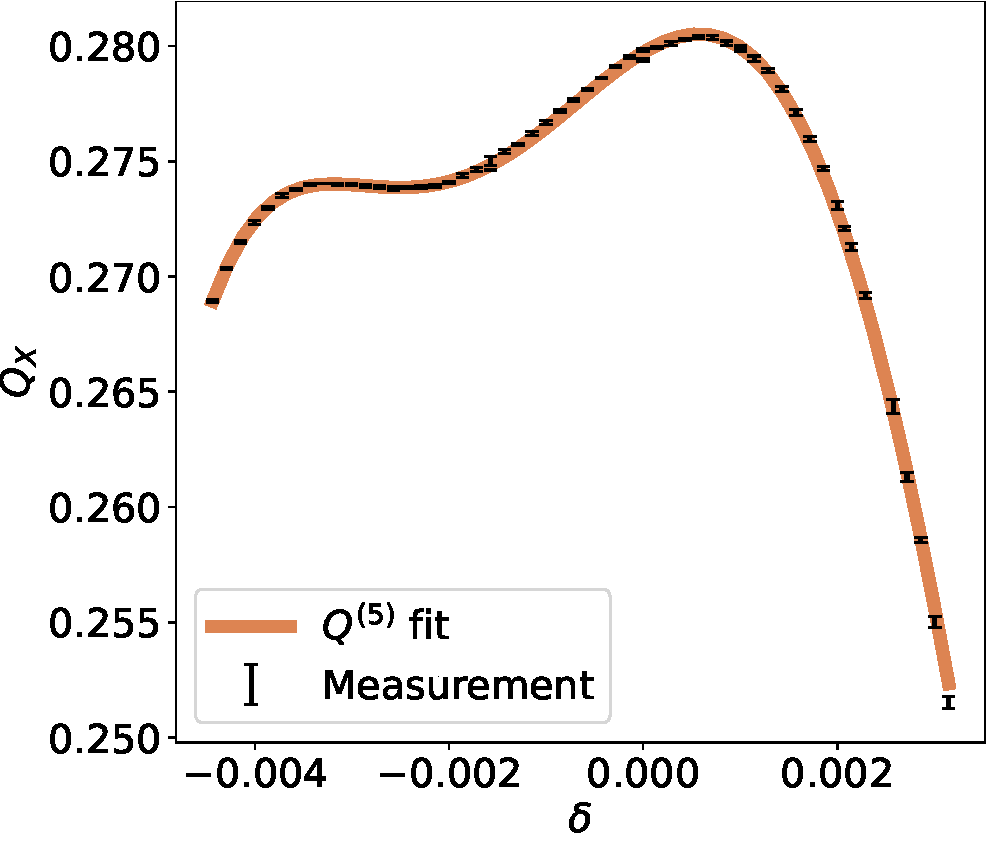
\includegraphics[width=\textwidth]{./images/chromaticity_further/q5_range/Beam2_Qx_full_but_not_quite.pdf}
        \caption{$Q_x$ Beam 2 High Range}
    \end{subfigure}
    \hfill
    \begin{subfigure}{0.49\textwidth}
        \centering
        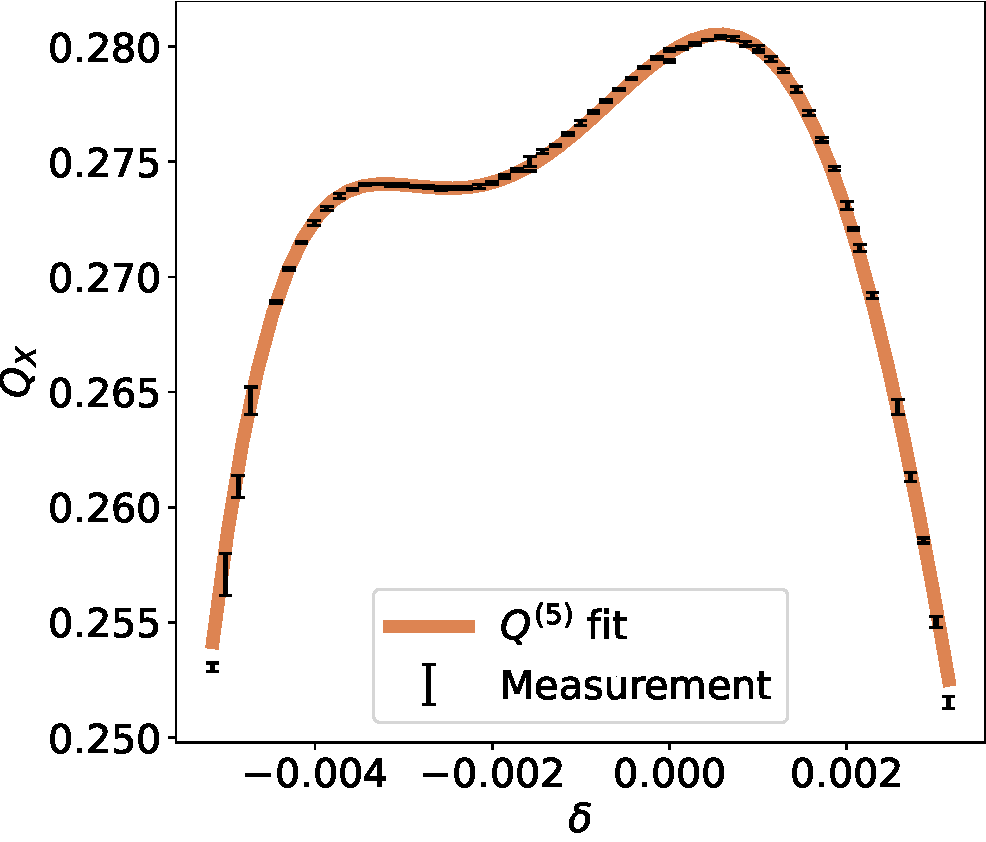
\includegraphics[width=\textwidth]{./images/chromaticity_further/q5_range/Beam2_Qx_full.pdf}
        \caption{$Q_y$ Beam 2 Full Range}
    \end{subfigure}
    %
    \caption{Third Beam 2 measurement of \cref{table:high_orders:dpp_ranges} with nominal
    corrections. A very large momentum offset range clearly highlights the non-linearity of the
    chromaticity function.}
    \label{fig:high_orders:chroma_nominal_correction_full_range}
\end{figure}

\begin{table}[!htb]
    \centering
    \begin{tabular}{lcccc}
      \toprule
      Plane & $Q^{(2)} [\times 10^{3}]$ & $Q^{(3)} [\times 10^{6}]$ & $Q^{(4)} [\times 10^{9}]$ & $Q^{(5)} [\times 10^{12}]$ \\
      \midrule
      X &&&& \\  
      \hspace{2mm}Rest. Range &$-2.93 \pm 0.05$ & $-4.40 \pm 0.08$ & $-0.53 \pm 0.08$ & $ 1.66 \pm 0.16$ \\
      \hspace{2mm}High Range  &$-2.99 \pm 0.05$ & $-4.71 \pm 0.03$ & $-0.42 \pm 0.07$ & $ 2.23 \pm 0.07$ \\
      \hspace{2mm}Full Range  &$-3.05 \pm 0.05$ & $-4.75 \pm 0.03$ & $-0.33 \pm 0.07$ & $ 2.34 \pm 0.06$ \\
      Y &&&& \\  
      \hspace{2mm}Rest. Range &$ 0.89 \pm 0.02$ & $ 2.05 \pm 0.03$ & $ 0.32 \pm 0.03$ & $-0.73 \pm 0.06$ \\
      \hspace{2mm}High Range  &$ 0.87 \pm 0.02$ & $ 2.07 \pm 0.02$ & $ 0.36 \pm 0.03$ & $-0.77 \pm 0.03$ \\
      \hspace{2mm}Full Range  &$ 0.70 \pm 0.04$ & $ 1.83 \pm 0.03$ & $ 0.64 \pm 0.06$ & $-0.32 \pm 0.05$ \\
      \bottomrule
    \end{tabular}
    \caption{Variance of the chromaticity values depending on the considered momentum offset range.
    All ranges have an upper bound of $3.2\times10^{-3}$. The lower bounds are, in order of
    appearance: $-3.5$, $-4.5$, $-5.2$.}
    \label{tab:high_orders:further:chroma_different_ranges}
  \end{table}

\Cref{tab:high_orders:further:chroma_different_ranges} shows the obtained chromaticity values for
varying ranges. From this table, it can be noted that increasing the range mainly
changes the estimate for $Q^{(5)}_x$.
Measurements over such a wide range are not yet fully understood, as other non-linear effects can
induce a detuning. For example, transverse impedances leads to a defocusing effect whose magnitude
increases with the orbit offset~\cite{antipov_single-collimator_2018,kurtulus_lhc_2022}.
Some other performed measurements with wide ranges in 2024 could not be fitted with a chromaticity
function, despite including higher orders. It is deemed that restricting the ranges is beneficial to
the fit estimates, until further investigation of these effects.



% --------------------------------
%       Even Higher Orders?
\subsubsection{\review{Higher Orders}}

The fifth measurement in \cref{table:high_orders:dpp_ranges} covered a range of $[-4.0 \cdot
10^{-3}, 4.5 \cdot 10^{-3}]$, which is among the widest ever measured. It is clear from
\cref{fig:high_orders:chroma_after_correction_full_range} that a chromaticity function including the
sixth order provides a better fit to the data. However, no additional observations were made for
this order, and considering the previously mentioned limitations, this measurement may not be
entirely robust. Further studies could address these limitations to more accurately characterize the
decahexapolar fields of the LHC at injection energy.

\begin{figure}[!htb]
    \begin{subfigure}{0.49\textwidth}
        \centering
        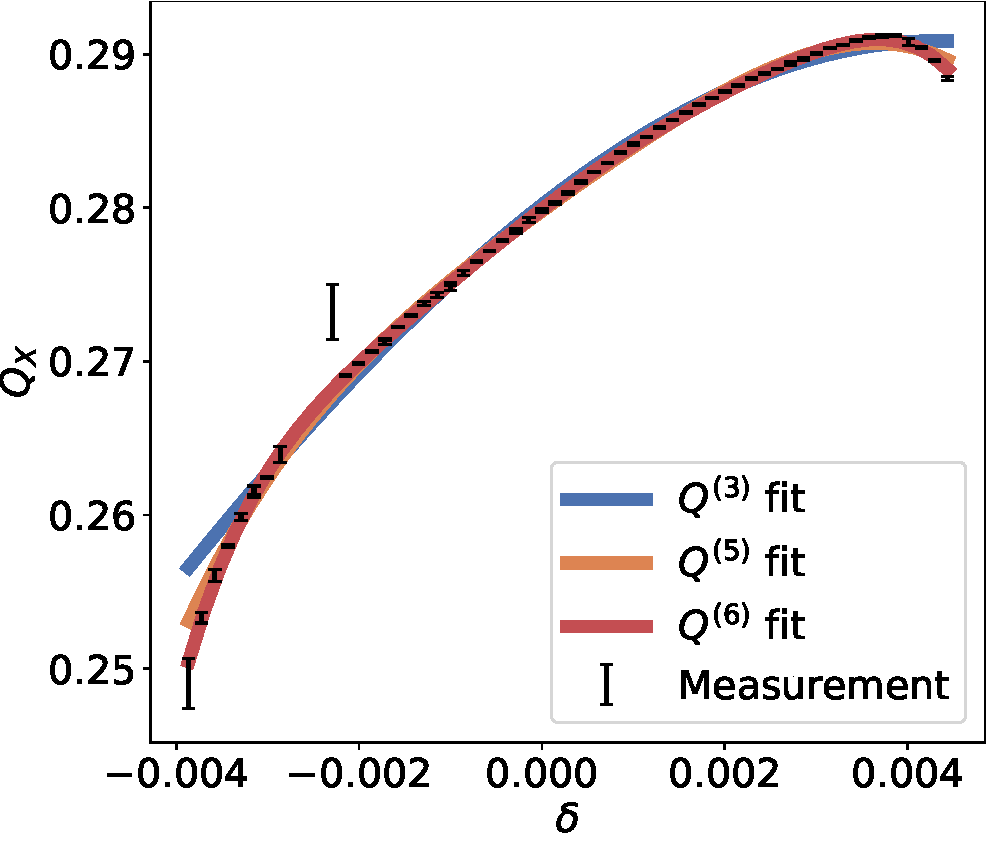
\includegraphics[width=\textwidth]{./images/chromaticity_further/q6/Beam1_Qx.pdf}
        \caption{$Q_x$ Beam 1}
    \end{subfigure}
    \hfill
    \begin{subfigure}{0.49\textwidth}
        \centering
        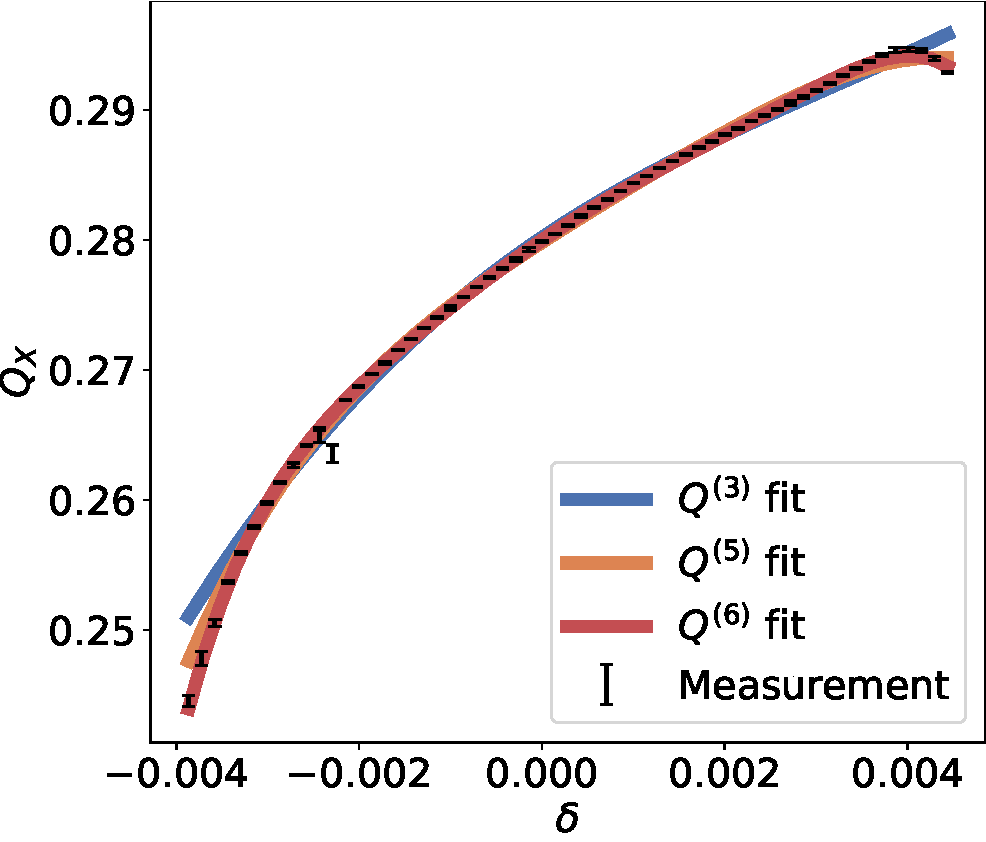
\includegraphics[width=\textwidth]{./images/chromaticity_further/q6/Beam2_Qx.pdf}
        \caption{$Q_x$ Beam 2}
    \end{subfigure}
    %
    \caption{Fifth measurement of \cref{table:high_orders:dpp_ranges} with $Q''$ and $Q'''$
    corrections. A possible sixth chromaticity order can be seen.}
    \label{fig:high_orders:chroma_after_correction_full_range}
\end{figure}




% --------------------------------
%          RDT
% --------------------------------
\subsection{\todo{Resonance Driving Terms}}

corrections? relevance? DA? 


%=============================
%        Conclusion
%=============================
\section{\todo{Summary}}

A wider momentum offset range, combined with new analysis techniques permitted the observation of
the fourth and fifth order of the chromaticity function for the first time in the LHC. Reproducible
values were measured with different machine configurations.

Simulations show that the observed values do not match well with the LHC non-linear model. A factor
$\approx 1.5$ is observed between measurements and simulations for $Q^{(5)}$, which may point to a
systematic error in the b7 error model.

Correction of the measured higher order chromaticity terms is not possible, due to the lack of
adequate correctors in the LHC. It is nevertheless interesting to characterize the higher order
errors for an effective model and understand the effect a higher order fit has on lower order terms.
Precise measurement of those lower chromaticity terms is required in order to effectively correct
them. Higher order terms have thus to be taken into account.

The current range of momentum offset is deemed sufficient to measure higher order chromaticity.
Attempts will, however, be taken to increase that range and assess if such a wider range can refine
the estimate of $Q^{(4)}$ and $Q^{(5)}$.